%!TEX ROOT = thesis.tex

\chapter{Semantics Retrieval Engine, Results and Analysis}

\label{section:retrievalengine}
\section{Introduction}

As described in Section~\ref{section:introduction}, there's an evident gap between the process of obtaining user described events and the retrieval of the desired video shots. Traditional approach of collecting text-based description of events alone are insufficient for effective retrieval process. With the vehicle-specific features such as the vehicle trajectory, time-stamp information, and colour information extracted via the extraction module introduced in Chapter~\ref{section:semanticsextraction}, retrieval techniques were designed to retrieve video shots resembling user described queries. This chapter engages the topic of semantic retrieval engines in detail and evaluates their performances along with analysis of the end results.

In this chapter, two retrieval techniques with relatively different concepts and underlying frameworks are discussed. The first technique was designed with a classic document retrieval system in mind, while the second technique was developed in order to address the shortcomings of the first. This is then followed by the methods used to measure the difference between the user-described trajectory, methods used to classify the vehicle colour, scoring systems used along with the results based on multiple user's review of the proposed method. This chapter also includes the speed measurement of the second retrieval engine.

As described in the Experimental Methodology (see~\ref{sec:expmethodology}), both the vehicle trajectory and vehicle colour evaluation process were separated in order to better gauge the performance of each technique.

\section{\versionOneRet}
\label{section:versionOne}
This section uncovers the techniques used behind this retrieval engine's framework along with the results. As previously introduced, this retrieval engine was inspired by Locality Sensitive Hashing (LSH) where documents are hashed into similar locations depending on the similarity. With that in mind,  the concept of this retrieval engine is first discussed. Next, the scoring system is introduced followed by the evaluation of the system in the following subsections.

\subsection{Concept}
\label{versionOneConcept}
By taking advantage of the spatio-temporal atom cubes structure introduced in Chapter~\ref{section:atoms}, each catalogued event in an atom were treated as an unique document. The underlying atom-based structure allows queries to be formed in a way which emulates the semantics extraction process. Hence, this eliminates the need for query parsing which in turn reduces the need of both pre- and post-processing of the given queries.

In this setup, each document containing similar contents were placed in the same SQL table as a mode of clustering documents. An example is given in Table~\ref{table:dbSample} to provide better visualisation of the proposed method. These sequence of events is also visualised in Figure~\ref{fig:motionExample} with the trajectory marked with \textcircled{2}.
In the example, a red vehicle was detected frame 180 to 184 of a video file on the 19th of March 2016 at 8:51:00am until 8:51:05am, from atom location (3,15) to (5,17) but was detected as a pink vehicle at frame 181.
The time information from frame $\mathbb{T}$ can be deduced using $\mathbb{T}_{time}  = (\mathbb{VD} \times \frac{\mathbb{T}}{\mathbb{TF}}) + \mathbb{F}_{time}$ where $\mathbb{VD}$ corresponds to the video duration of each file (6 minutes) and $\mathbb{TF}$ is the total frames of the current video. The $\mathbb{F}_{time}$ is the time information extracted from filename.
Hence, the current frame time at frame 181 is obtained as such: $(6_{minutes} \times \frac{181}{360}) + 08:48:00am = 8:51:01am$.

As each catalogued event is treated as a unique document (a single record in the database) in this framework, the retrieval process begins by filtering out tables which are irrelevant to the query, $\mathbb{Q}$. Falling back on the example given in Table~\ref{table:dbSample}, the system is able to effectively skip through 9 colour tables and 5 motion tables, hence speeding up the process to locate documents of interest while reducing the overhead cost involved when going through an entire database. Upon filtering out irrelevant tables, the retrieval engine proceeds to extract and group up all the relevant records according to the filenames.

Next, the retrieved results are validated to see if they belong to the same vehicle by cross-checking the obj\_id. Along with that, the retrieval engine also validates if the results belong to a similar time-frame by comparing the t-coordinate. This step is essential to ensure that each result belongs to the same vehicle trajectory group as the initial tracker may re-assign a obj\_id to another vehicle during the background subtraction process.
While the results returned at this point were accurate, one major problem that occurs using the current process is the low recall rate. The recall rate in a retrieval engine can be thought as the percentage of relevant documents which were retrieved over the total amount of relevant documents; while a low recall rate is preferable in an environment where the accuracy of the retrieved result is regarded with high importance and false negatives are welcomed over false positive such as the medical industry, this is not the case in the proposed method.

In order to overcome the limitation of the low recall rate, a Confidence Value (CV) score parameter is introduced. The CV parameter was used to adjust the sensitivity level of accepting a video shot as part of the final retrieved results. In the proposed method, a lower CV would return a larger set of results at the expense of an increase of retrieved shots which may or may not improve the overall accuracy of the retrieval engine. Each retrieved shot, $\mathbb{S}_i$, will be accepted as the final retrieved results if it fulfils the condition in Equation \ref{eq:CVscore}. The use of the CV score parameter provides a margin of error when performing the query which acts as a trade-off function.

\begin{equation}
\label{eq:CVscore}
CV < \frac{\text{length}(\mathbb{S}_i)}{\text{length}(\mathbb{Q})} \times 100\%
\end{equation}



Upon validating the sanctity of the results, commands were sent to FFmpeg to extract the video shots based on the given filename along with the start and end frame number. Finally, the users are presented with the output from the retrieval engine where the final results can be viewed.


% Please add the following required packages to your document preamble:
% \usepackage[normalem]{ulem}
\begin{table}[!hbt]
	\centering
\caption{Database Structure for a Vehicle Identified as Red and Pink Colour with Object id "1" of the \versionOneRet }
\label{table:dbSample}
\begin{tabular}{llllll}
\multicolumn{6}{l}{{ colour\_red}} \\ \hline
\multicolumn{1}{|l|}{\textbf{row\_id}} & \multicolumn{1}{l|}{\textbf{filename}}    & \multicolumn{1}{l|}{\textbf{obj\_id}} & \multicolumn{1}{l|}{\textbf{atom\_x}} & \multicolumn{1}{l|}{\textbf{atom\_y}} & \multicolumn{1}{l|}{\textbf{atom\_t}} \\ \hline
\multicolumn{1}{|l|}{n}                & \multicolumn{1}{l|}{20160319\_084800.mp4} & \multicolumn{1}{l|}{1}                & \multicolumn{1}{l|}{3}                & \multicolumn{1}{l|}{15}               & \multicolumn{1}{l|}{180}              \\ \hline
\multicolumn{1}{|l|}{n+1}              & \multicolumn{1}{l|}{20160319\_084800.mp4} & \multicolumn{1}{l|}{1}                & \multicolumn{1}{l|}{3}                & \multicolumn{1}{l|}{16}               & \multicolumn{1}{l|}{182}              \\ \hline
\multicolumn{1}{|l|}{n+2}              & \multicolumn{1}{l|}{20160319\_084800.mp4} & \multicolumn{1}{l|}{1}                & \multicolumn{1}{l|}{4}                & \multicolumn{1}{l|}{16}               & \multicolumn{1}{l|}{183}              \\ \hline
\multicolumn{1}{|l|}{n+3}              & \multicolumn{1}{l|}{20160319\_084800.mp4} & \multicolumn{1}{l|}{1}                & \multicolumn{1}{l|}{5}                & \multicolumn{1}{l|}{17}               & \multicolumn{1}{l|}{184}              \\ \hline
                                       &                                           &                                       &                                       &                                       &                                       \\
\multicolumn{6}{l}{{ colour\_pink}}                                                                                                                                                                                                              \\ \hline
\multicolumn{1}{|l|}{\textbf{row\_id}} & \multicolumn{1}{l|}{\textbf{filename}}    & \multicolumn{1}{l|}{\textbf{obj\_id}} & \multicolumn{1}{l|}{\textbf{atom\_x}} & \multicolumn{1}{l|}{\textbf{atom\_y}} & \multicolumn{1}{l|}{\textbf{atom\_t}} \\ \hline
\multicolumn{1}{|l|}{m}                & \multicolumn{1}{l|}{20160319\_084800.mp4} & \multicolumn{1}{l|}{1}                & \multicolumn{1}{l|}{3}                & \multicolumn{1}{l|}{16}               & \multicolumn{1}{l|}{181}              \\ \hline
                                       &                                           &                                       &                                       &                                       &                                       \\
\multicolumn{6}{l}{{ direction\_down}}                                                                                                                                                                                                          \\ \hline
\multicolumn{1}{|l|}{\textbf{row\_id}} & \multicolumn{1}{l|}{\textbf{filename}}    & \multicolumn{1}{l|}{\textbf{obj\_id}} & \multicolumn{1}{l|}{\textbf{atom\_x}} & \multicolumn{1}{l|}{\textbf{atom\_y}} & \multicolumn{1}{l|}{\textbf{atom\_t}} \\ \hline
\multicolumn{1}{|l|}{h}                & \multicolumn{1}{l|}{20160319\_084800.mp4} & \multicolumn{1}{l|}{1}                & \multicolumn{1}{l|}{3}                & \multicolumn{1}{l|}{15}               & \multicolumn{1}{l|}{181}              \\ \hline
                                       &                                           &                                       &                                       &                                       &                                       \\
\multicolumn{6}{l}{{ direction\_motionless}}                                                                                                                                                                                                    \\ \hline
\multicolumn{1}{|l|}{\textbf{row\_id}} & \multicolumn{1}{l|}{\textbf{filename}}    & \multicolumn{1}{l|}{\textbf{obj\_id}} & \multicolumn{1}{l|}{\textbf{atom\_x}} & \multicolumn{1}{l|}{\textbf{atom\_y}} & \multicolumn{1}{l|}{\textbf{atom\_t}} \\ \hline
\multicolumn{1}{|l|}{j}                & \multicolumn{1}{l|}{20160319\_084800.mp4} & \multicolumn{1}{l|}{1}                & \multicolumn{1}{l|}{3}                & \multicolumn{1}{l|}{16}               & \multicolumn{1}{l|}{182}              \\ \hline
                                       &                                           &                                       &                                       &                                       &                                       \\
\multicolumn{6}{l}{{ direction\_right}}                                                                                                                                                                                                         \\ \hline
\multicolumn{1}{|l|}{\textbf{row\_id}} & \multicolumn{1}{l|}{\textbf{filename}}    & \multicolumn{1}{l|}{\textbf{obj\_id}} & \multicolumn{1}{l|}{\textbf{atom\_x}} & \multicolumn{1}{l|}{\textbf{atom\_y}} & \multicolumn{1}{l|}{\textbf{atom\_t}} \\ \hline
\multicolumn{1}{|l|}{k}                & \multicolumn{1}{l|}{20160319\_084800.mp4} & \multicolumn{1}{l|}{1}                & \multicolumn{1}{l|}{3}                & \multicolumn{1}{l|}{16}               & \multicolumn{1}{l|}{183}              \\ \hline
                                       &                                           &                                       &                                       &                                       &                                       \\
\multicolumn{6}{l}{{ direction\_right\_down}}                                                                                                                                                                                                   \\ \hline
\multicolumn{1}{|l|}{\textbf{row\_id}} & \multicolumn{1}{l|}{\textbf{filename}}    & \multicolumn{1}{l|}{\textbf{obj\_id}} & \multicolumn{1}{l|}{\textbf{atom\_x}} & \multicolumn{1}{l|}{\textbf{atom\_y}} & \multicolumn{1}{l|}{\textbf{atom\_t}} \\ \hline
\multicolumn{1}{|l|}{l}                & \multicolumn{1}{l|}{20160319\_084800.mp4} & \multicolumn{1}{l|}{1}                & \multicolumn{1}{l|}{3}                & \multicolumn{1}{l|}{16}               & \multicolumn{1}{l|}{184}              \\ \hline
\end{tabular}
\end{table}

\subsection{Search Interface}

The proposed retrieval engine was realised in a form of a graphical user search interface written in C++, where users are able to construct queries by drawing the trajectory on the interface and providing complementary query information such as the vehicle colour. With these user-described query information, the user can then perform queries and obtain the results within seconds. Figure \ref{fig:versionOneInterface} shows the proposed interface with the green lines indicating the user-described trajectory as the query. Upon processing the results, FFmpeg will then extract the video shots and populate the results in a folder.





\begin{figure}[!htb]
	\centering
	\begin{tabular}{c}
		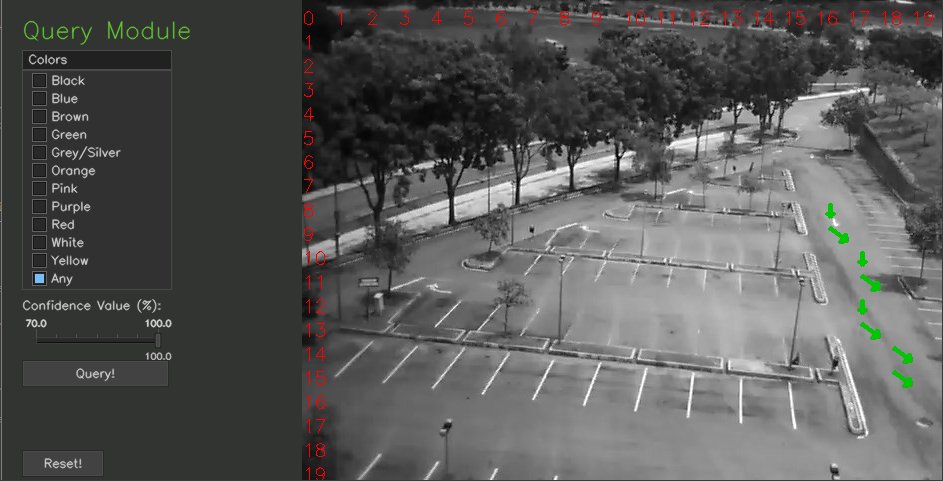
\includegraphics[width=0.7\linewidth]{image/retrievalOne/test1-8inputs.PNG} \\
		(a) Motion Test Case 1 (TQ1) \\
		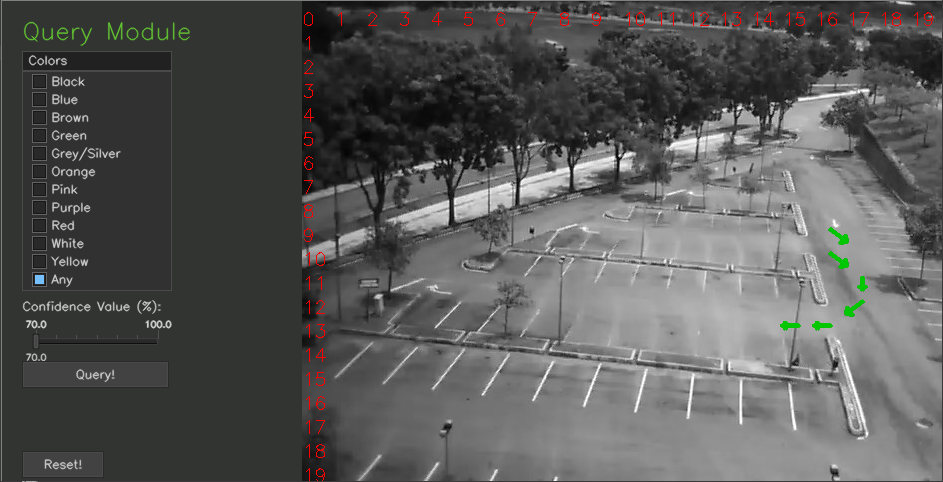
\includegraphics[width=0.7\linewidth]{image/retrievalOne/test2-6input.PNG}\\
		(b) Motion Test Case 2 (TQ2)
	\end{tabular}
	\caption{Search Interface for \versionOneRet}
	\label{fig:versionOneInterface}
\end{figure}




\subsection{Results and Analysis}
The following subsections describes the evaluation process of the proposed method in Section \ref{section:semantic_lsh} which includes both the vehicle trajectory as well as the vehicle colour. As previously mentioned in Section \ref{sec:expmethodology}, only two days of data were fully annotated with the number of vehicles with their corresponding colour (see Table \ref{table:colorDist}) as well as the total number of vehicles that performed both $TQ1$ and $TQ2$.

With the annotated values, the Precision and Recall (Equation \ref{eq:precisionrecall}) metrics were used to measure the performance of the proposed method. These values can be calculated as the total number of event occurrence were recorded; hence, the $F_1$ score can also be computed (Equation \ref{eq:f1score}). The precision of a retrieval engine can be thought as the ratio between number of accurate results over the total number of retrieved results. The recall, on the hand, indicates the ratio of relevant results which were retrieved over the total retrieved results. Finally, the $F_1$ score is used as a harmonic mean between both Precision and Recall values which are both desirable in a retrieval engine.

\begin{align}
\label{eq:precisionrecall}
    \text{Precision} = \frac{tp}{tp + fp}   \hspace{1em} \text{ ; }  \hspace{1em} \text{Recall}  = \frac{tp}{tp + fn}
\end{align}
\begin{align}
\label{eq:f1score}
\text{F1-score}  = 2\cdot\frac{\text{Precision} \cdot \text{Recall}}{\text{Precision} + \text{Recall}}
\end{align}



\subsubsection{Vehicle Trajectory}

In order to evaluate the performance of the retrieval engine in regards to vehicle trajectories, the ground truth of the data has to be first obtained. As the manual annotation of these video data is laborious and time consuming, only two specific motion paths were designated as trajectory queries (TQ). The first query, TQ1 refers to vehicles heading southward (see Figure \ref{fig:versionOneInterface} (a)) while TQ2 represents vehicles turning into a junction (see Figure \ref{fig:versionOneInterface} (b)).

These predefined trajectory queries (TQ) were selected to represent two types of motion which exist in a car park scene, (i) \textit{simple motion} - motions that are simple in nature, moving straight \& (ii) \textit{complex motion} - motions which contains multiple elements such as turning into a junction. The distribution of these TQ are tabulated in Table \ref{table:motiondist}. In each TQ experiment, the number of atom input query used to represent each TQ were varied to understand the co-relating effects between the number of inputs and the performance of the retrieval engine. In addition to that, the effects of using varying confidence values (CV) in regards to the performance is also evaluated. These experiments were tested on three CV values which were set at 70\%, 80\%, and 90\%.


\begin{table}[bht!]
\centering
\caption{Ground Truth Distribution of Trajectory Queries}
\label{table:motiondist}
\begin{tabular}{cccc}
\toprule
Trajectory Query &  Trajectory Type & \# of Occurrence & Distribution (\%)   \\
\midrule
TQ1       & Simple Motion       & 252 & 86.3   \\
TQ2      & Complex Motion       & 40 & 13.7  \\
\bottomrule
\end{tabular}
\end{table}

Based on the results tabulated in Table \ref{table:motionResults}, the average precision of both TQ1 and TQ2 using CV at 70\% is 67.64\%. The increase of CV to 70\% to 90\% shows an increase in terms of average precision. For TQ1, the average precision increased from 89.50\% to 89.51\% and finally 90.49\% when CV was set at 90\% with a total increase of approximately 1\% for the precision metrics. Likewise, for TQ2, the average precision showed a total increase of 7.44\% when then CV parameter was tweaked. The average precision increased from 45.79\% to 52.61\% and reaching 53.23\% when CV was set to 90\%.

However, the recall metrics showed a different side of the story when the average recall rate fell from 39.67\% to 18.01\% for TQ1 and 68.15\% to 51.85\% for TQ2. This drastic drop in for recall metrics shows direct co-relation with the requirement of fulfilling Equation \ref{eq:CVscore} for each retrieved shots. The results shows consistency throughout the various experimental settings and true towards the concept which was introduced in \ref{versionOneConcept}.

As a whole, the $F_1$ score metric was used to evaluate the overall performance of the proposed method as it provides a balance between both of the desirable metrics discussed above. Based on the results, queries with the lowest CV and lower number of inputs tend to perform better than the other parameter settings. The proposed method was able to achieve an $F_1$ score of 74.32\% and 68.08\% for both TQ1 and TQ2.


\begin{table}[tb!]
\centering
\caption{Results of Motion Retrieval Task with Varying CV and Number of Atom Inputs}
\label{table:motionResults}
\vspace{0.5em}
\resizebox{\textwidth}{!}{
\begin{tabular}{ccc|c|c|c|c|c|c|c|c|c|}
\cline{4-12}
\cline{4-12}
& & & \multicolumn{3}{c|}{CV: 70\%} & \multicolumn{3}{c|}{CV: 80\%} & \multicolumn{3}{c|}{CV: 90\%} \\ \cline{4-12}
 & & & Precision & Recall & F1 Score & Precision & Recall & F1 Score & Precision & Recall & F1 Score \\ \hline
\multicolumn{1}{|c|}{\multirow{7}{*}{\rotatebox[origin=c]{90}{No. of Input}}} & \multicolumn{1}{c|}{\multirow{4}{*}{\rotatebox[origin=c]{90}{TQ1}}} & 5 & 93.82 & 61.53  & \cellcolor[HTML]{32CB00}\textbf{74.32} & 95.34 & 33.19  & 49.24 & 95.34 & 33.19 & 49.24   \\ \cline{3-12}
\multicolumn{1}{|c|}{} & \multicolumn{1}{c|}{} & 6 & 90.09 & 36.84 & 52.29 & 90.09 & 36.84  & 52.29 & 89.13 & 16.59 & 27.98    \\ \cline{3-12}
\multicolumn{1}{|c|}{} & \multicolumn{1}{c|}{} & 7 & 87.27 & 38.86 & 53.78 & 88 & 17.81  & 29.62 & 87.87 & 11.74 & 20.71    \\ \cline{3-12}
\multicolumn{1}{|c|}{} & \multicolumn{1}{c|}{} & 8 & 86.88 & 21.45 & 34.41 & 84.61 & 13.36  & 23.07 & 89.65 & 10.52 & 18.84    \\ \cline{2-12}
\multicolumn{1}{|c|}{} & \multicolumn{1}{c|}{\multirow{3}{*}{\rotatebox[origin=c]{90}{TQ2}}} & 4 & 16.28 & 80 & 27.06 & 28.69 & 73.33  & 41.25    & 28.69 & 73.33 & 41.25    \\ \cline{3-12}
\multicolumn{1}{|c|}{} & \multicolumn{1}{c|}{} & 5 & 65.3 & 71.11  & \cellcolor[HTML]{32CB00}\textbf{68.08} & 73.33 & 48.88  & 58.66 & 73.33 & 48.88  & 58.66    \\ \cline{3-12}
\multicolumn{1}{|c|}{} & \multicolumn{1}{c|}{} & 6 & 55.81 & 53.33 & 54.54 & 55.81 & 53.33 & 54.54 & 57.69 & 33.33 & 42.25    \\ \hline
\end{tabular}}
\end{table}




\subsubsection{Vehicle Colour}

\begin{table}[bht!]
\centering
\caption{Ground Truth Distribution Vehicle Colours Ordered by Occurrence}
\label{table:colorDist}
\begin{tabular}{ccc}
\toprule
Colour Term & \# of Occurrence & Distribution (\%)   \\
\midrule
Gray       & 365       & 43.61  \\
Black      & 182       & 21.74  \\
White      & 150       & 17.92  \\
Red        & 60        & 7.17   \\
Blue       & 19        & 2.27   \\
Orange     & 15        & 1.79   \\
Yellow     & 13        & 1.55   \\
Green      & 10        & 1.19   \\
Pink       & 9         & 1.08   \\
Purple     & 7         & 0.84   \\
Brown      & 7         & 0.84   \\
\bottomrule
\end{tabular}
\end{table}




The results of the proposed colour term extraction algorithm (\ref{algo:colorExtract}) is tabulated in Table \ref{table:colorMatrix} in a form of a confusion matrix. The cells which are marked in green refers to vehicles which were correctly predicted with the highest count, while cells which are marked in red refers to the highest count of incorrect predictions. The overall performance in terms of precision is around 54\% while the recall is reported at around 36\% with the $F_1$ score of 39\%. The tabulated results also shows that approximately 12\% of vehicles were wrongly classified as achromatic vehicles which were affected by the proposed $T_{pivot}$ value. However, when setting aside the performance of the algorithm to differentiate between chromatic and achromatic vehicles, the proposed method was able to predict the colour classes for seven out of eleven colour classes. Nevertheless, the results were taken with a grain of salt as the number of test case for each of those colour classes were rather low for a decisive verdict.

Next, the performance of the proposed Algorithm \ref{algo:achromatic} using white and black filters as an approach towards differentiating between all three achromatic colours was analysed. The proposed algorithm performed relatively well with an average accuracy of 68\%. The results shows that the proposed algorithm did not have much trouble differentiating between black and white vehicles, however, the algorithm tend to have trouble classifying between gray-black and gray-white vehicles as they tend to be ambiguous depending on the lighting condition in the video data. As mentioned above, the $T_{pivot}$'s performance was not up to par. The pivoting process between chromatic and achromatic vehicles proves to be inefficient in harsh lighting condition where shadows and rain would drastically affect the outcome as vehicles may suffer from the lack of chromatic hues which is used to assist in the accurate prediction.

While better results could potentially be obtained by carefully and systematically tweaking the $T_{pivot}$ to perform better at distinguishing between chromatic and achromatic vehicles, the hand crafted parameter may not work well in other scenarios belonging to other dataset, hence, making it undesirable as it is not easily extensible. Another disadvantage of the proposed method used in this framework is that each colour had only one final predicted colour term. As an example, the predicted results for Red colour in Table \ref{table:colorMatrix} illustrates this issue where the colour term of three vehicles were assigned Pink instead of Red even though Red and Pink colour both belongs to the similar hues.


\begin{table}[!ht]
\centering
\caption{Confusion Matrix for Colour Retrieval Task}
\vspace{1.5em}
\label{table:colorMatrix}
\resizebox{\columnwidth}{!}{
\begin{tabular}{ccccccccccccc}
\cline{3-13}
 & \multicolumn{1}{l|}{} & \multicolumn{11}{c|}{Predicted Colour} \\ \cline{3-13}
 & \multicolumn{1}{c|}{} & \multicolumn{1}{c|}{Gray} & \multicolumn{1}{c|}{Black} & \multicolumn{1}{c|}{White} & \multicolumn{1}{c|}{Red} & \multicolumn{1}{c|}{Blue} & \multicolumn{1}{c|}{Orange} & \multicolumn{1}{c|}{Yellow} & \multicolumn{1}{c|}{Green} & \multicolumn{1}{c|}{Pink} & \multicolumn{1}{c|}{Purple} & \multicolumn{1}{c|}{Brown} \\ \hline
\multicolumn{1}{|l|}{} & \multicolumn{1}{c|}{Gray} & \multicolumn{1}{c|}{\cellcolor[HTML]{32CB00}\textbf{236}} & \multicolumn{1}{c|}{61} & \multicolumn{1}{c|}{68} & \multicolumn{1}{c|}{0} & \multicolumn{1}{c|}{0} & \multicolumn{1}{c|}{0} & \multicolumn{1}{c|}{0} & \multicolumn{1}{c|}{0} & \multicolumn{1}{c|}{0} & \multicolumn{1}{c|}{0} & \multicolumn{1}{c|}{0} \\ \cline{2-13}
\multicolumn{1}{|l|}{} & \multicolumn{1}{c|}{Black} & \multicolumn{1}{c|}{48} & \multicolumn{1}{c|}{\cellcolor[HTML]{32CB00}\textbf{134}} & \multicolumn{1}{c|}{0} & \multicolumn{1}{c|}{0} & \multicolumn{1}{c|}{0} & \multicolumn{1}{c|}{0} & \multicolumn{1}{c|}{0} & \multicolumn{1}{c|}{0} & \multicolumn{1}{c|}{0} & \multicolumn{1}{c|}{0} & \multicolumn{1}{c|}{0} \\ \cline{2-13}
\multicolumn{1}{|l|}{} & \multicolumn{1}{c|}{White} & \multicolumn{1}{c|}{26} & \multicolumn{1}{c|}{4} & \multicolumn{1}{c|}{\cellcolor[HTML]{32CB00}\textbf{120}} & \multicolumn{1}{c|}{0} & \multicolumn{1}{c|}{0} & \multicolumn{1}{c|}{0} & \multicolumn{1}{c|}{0} & \multicolumn{1}{c|}{0} & \multicolumn{1}{c|}{0} & \multicolumn{1}{c|}{0} & \multicolumn{1}{c|}{0} \\ \cline{2-13}
\multicolumn{1}{|l|}{} & \multicolumn{1}{c|}{Red} & \multicolumn{1}{c|}{27} & \multicolumn{1}{c|}{25} & \multicolumn{1}{c|}{0} & \multicolumn{1}{c|}{2} & \multicolumn{1}{c|}{0} & \multicolumn{1}{c|}{0} & \multicolumn{1}{c|}{0} & \multicolumn{1}{c|}{0} & \multicolumn{1}{c|}{4} & \multicolumn{1}{c|}{\cellcolor[HTML]{FE0000}\textbf{2}} & \multicolumn{1}{c|}{0} \\ \cline{2-13}
\multicolumn{1}{|l|}{} & \multicolumn{1}{c|}{Blue} & \multicolumn{1}{c|}{3} & \multicolumn{1}{c|}{10} & \multicolumn{1}{c|}{0} & \multicolumn{1}{c|}{0} & \multicolumn{1}{c|}{\cellcolor[HTML]{32CB00}\textbf{6}} & \multicolumn{1}{c|}{0} & \multicolumn{1}{c|}{0} & \multicolumn{1}{c|}{0} & \multicolumn{1}{c|}{0} & \multicolumn{1}{c|}{0} & \multicolumn{1}{c|}{0} \\ \cline{2-13}
\multicolumn{1}{|l|}{} & \multicolumn{1}{c|}{Orange} & \multicolumn{1}{c|}{8} & \multicolumn{1}{c|}{3} & \multicolumn{1}{c|}{0} & \multicolumn{1}{c|}{0} & \multicolumn{1}{c|}{0} & \multicolumn{1}{c|}{\cellcolor[HTML]{32CB00}\textbf{3}} & \multicolumn{1}{c|}{0} & \multicolumn{1}{c|}{0} & \multicolumn{1}{c|}{0} & \multicolumn{1}{c|}{1} & \multicolumn{1}{c|}{0} \\ \cline{2-13}
\multicolumn{1}{|l|}{} & \multicolumn{1}{c|}{Yellow}    & \multicolumn{1}{c|}{3} & \multicolumn{1}{c|}{1} & \multicolumn{1}{c|}{2} & \multicolumn{1}{c|}{0} & \multicolumn{1}{c|}{0} & \multicolumn{1}{c|}{0} & \multicolumn{1}{c|}{\cellcolor[HTML]{32CB00}\textbf{7}} & \multicolumn{1}{c|}{0} & \multicolumn{1}{c|}{0} & \multicolumn{1}{c|}{0} & \multicolumn{1}{c|}{0} \\ \cline{2-13}
\multicolumn{1}{|l|}{} & \multicolumn{1}{c|}{Green} & \multicolumn{1}{c|}{5} & \multicolumn{1}{c|}{1} & \multicolumn{1}{c|}{4} & \multicolumn{1}{c|}{0} & \multicolumn{1}{c|}{0} & \multicolumn{1}{c|}{0} & \multicolumn{1}{c|}{0} & \multicolumn{1}{c|}{\cellcolor[HTML]{C0C0C0}\textbf{0}} & \multicolumn{1}{c|}{0} & \multicolumn{1}{c|}{0} & \multicolumn{1}{c|}{0} \\ \cline{2-13}
\multicolumn{1}{|l|}{} & \multicolumn{1}{c|}{Pink} & \multicolumn{1}{c|}{1} & \multicolumn{1}{c|}{0} & \multicolumn{1}{c|}{0} & \multicolumn{1}{c|}{\cellcolor[HTML]{FE0000}\textbf{3}} & \multicolumn{1}{c|}{0} & \multicolumn{1}{c|}{0} & \multicolumn{1}{c|}{0} & \multicolumn{1}{c|}{0} & \multicolumn{1}{c|}{\cellcolor[HTML]{32CB00}\textbf{5}} & \multicolumn{1}{c|}{0} & \multicolumn{1}{c|}{0} \\ \cline{2-13}
\multicolumn{1}{|l|}{} & \multicolumn{1}{c|}{Purple} & \multicolumn{1}{c|}{3} & \multicolumn{1}{c|}{3} & \multicolumn{1}{c|}{0} & \multicolumn{1}{c|}{0} & \multicolumn{1}{c|}{0} & \multicolumn{1}{c|}{0} & \multicolumn{1}{c|}{0} & \multicolumn{1}{c|}{0} & \multicolumn{1}{c|}{0} & \multicolumn{1}{c|}{1} & \multicolumn{1}{c|}{0} \\ \cline{2-13}
\multicolumn{1}{|l|}{\multirow{-11}{*}{\rotatebox[origin=c]{90}{Actual Colour}}} & \multicolumn{1}{c|}{Brown} & \multicolumn{1}{c|}{3} & \multicolumn{1}{c|}{4} & \multicolumn{1}{c|}{0} & \multicolumn{1}{c|}{0} & \multicolumn{1}{c|}{0} & \multicolumn{1}{c|}{0} & \multicolumn{1}{c|}{0} & \multicolumn{1}{c|}{0} & \multicolumn{1}{c|}{0} & \multicolumn{1}{c|}{0} & \multicolumn{1}{c|}{\cellcolor[HTML]{C0C0C0}\textbf{0}} \\ \hline
 & \multicolumn{1}{l}{} & \multicolumn{1}{l}{} & \multicolumn{1}{l}{} & \multicolumn{1}{l}{} & \multicolumn{1}{l}{} & \multicolumn{1}{l}{} & \multicolumn{1}{l}{} & \multicolumn{1}{l}{} & \multicolumn{1}{l}{} & \multicolumn{1}{l}{} & \multicolumn{1}{l}{} & \multicolumn{1}{l}{} \\ \hline
\multicolumn{1}{|l|}{} & \multicolumn{1}{c|}{Precision} & \multicolumn{1}{c|}{65.01} & \multicolumn{1}{c|}{54.47}                                & \multicolumn{1}{c|}{61.86} & \multicolumn{1}{c|}{40.00} & \multicolumn{1}{c|}{100.00} & \multicolumn{1}{c|}{100.00}                             & \multicolumn{1}{c|}{100.00} & \multicolumn{1}{c|}{N/A} & \multicolumn{1}{c|}{55.56} & \multicolumn{1}{c|}{25.00}                              & \multicolumn{1}{c|}{N/A} \\ \cline{2-13}
\multicolumn{1}{|l|}{} & \multicolumn{1}{c|}{Recall} & \multicolumn{1}{c|}{64.66} & \multicolumn{1}{c|}{73.63} & \multicolumn{1}{c|}{80.00} & \multicolumn{1}{c|}{3.33} & \multicolumn{1}{c|}{31.58} & \multicolumn{1}{c|}{20.00} & \multicolumn{1}{c|}{53.85} & \multicolumn{1}{c|}{0.00} & \multicolumn{1}{c|}{55.56} & \multicolumn{1}{c|}{14.29} & \multicolumn{1}{c|}{0.00} \\ \cline{2-13}
\multicolumn{1}{|l|}{\multirow{-3}{*}{\rotatebox[origin=c]{90}{Result}}} & \multicolumn{1}{c|}{F1 Score}  & \multicolumn{1}{c|}{64.84} & \multicolumn{1}{c|}{62.62} & \multicolumn{1}{c|}{69.77} & \multicolumn{1}{c|}{6.15} & \multicolumn{1}{c|}{48.00} & \multicolumn{1}{c|}{33.33} & \multicolumn{1}{c|}{70.00} & \multicolumn{1}{c|}{N/A} & \multicolumn{1}{c|}{55.56} & \multicolumn{1}{c|}{18.18} & \multicolumn{1}{c|}{N/A} \\ \hline
\end{tabular}%
}
\end{table}


% However, the current implementation of the proposed method search interface has yet to include time slicing query options.

%However, should the initial test against the $T_{pivot}$ fails, the proposed method is able to fall back on the HSV histogram results.


\section{\versionTwoRet}
\label{section:versionTwo}

This section expounds on the techniques used behind this retrieval engine's framework along with the results. The proposed interface in \versionTwoRet also focuses on extensibility as well as ease of access of the retrieval engine while improving on the overall results. The JavaScript (JS) language was selected as a means to this end as it is commonly used in web browsers. The focus of this work sees a shift from indexing methods to results-sorting optimisation by measuring the difference between the query and the retrieved results. The concept and scoring systems used in this retrieval engine will be discussed further in the following subsections along with the evaluation.

\subsection{Concept}

Instead of treating each spatio-temporal atom cubes as an unique document, in this framework, the unique identifiers ($atom_x$, $atom_y$, $atom_t$) of each atom was used in the retrieval process. As mentioned above, the focus of this framework veered towards the use of distance measures (see Section \ref{section:distancemeasures}) and its applications in order to retrieve results that are relevant.

In the same manner as the semantic extraction process, the graphical input query was designed in such a way that it takes on the properties of the atom cubes' unique identifiers with the exception of the $atom_t$. As a substitute of the identifier, the order of the input, $o_{i}$, was used as a replacement. This was possible as the order was used to mimic the motion of the target vehicle shot. However, to do so, first, the graphical query input needs to be converted into a set, $\mathbb{Q}$, by removing duplicate identifiers which was introduced by the mouse input strokes. This will thus result with unique identifiers remaining in the set.
\begin{equation}
    \mathbb{Q} = \{ (x_i, y_i, o_i), (x_{i+1}, y_{i+1}, o_{i+1}), (x_{i+2}, y_{i+2}, o_{i+2}), \dotsb,(x_{i+n}, y_{i+n}, o_{i+n})\}
\end{equation}
As the retrieval engine deals with a huge set of data, the next logical approach was to find ways to optimise and minimise the search area. In this framework, a simplistic approach was taken to further narrow down the search scope.
The time and date semantics were utilised as these useful metadata which were extracted during the semantic extraction phase were suitable candidates in assisting the filtering process.
Records $\mathbb{R}$ that fulfils the input query's requirements were kept and included into a set $\mathbb{P}$, while records which failed was filtered out from this phase using Equation \ref{eq:timedatefilter}.
\begin{gather}
\label{eq:timedatefilter}
     \text{Start Timestamp} \hspace{.5em} \leq \hspace{.5em} \mathbb{R}[i] \hspace{.5em} \leq \hspace{.5em} \text{End Timestamp} \hspace{.5em} \Rightarrow \hspace{.5em} \mathbb{R}[i] \in \mathbb{P}
\end{gather}
Now, with the output $\mathbb{P}$ from the filtering process, these records can now be compared against the input query $\mathbb{Q}$. In order to do so, this step begins by first comparing the length of the query ($\mathbb{Q}_{length}$) against the length of the individual records ($\mathbb{R}[i]_{length}$) in $\mathbb{P}$. This comparison is essential for the next phase of measuring the dissimilarity between using Chamfer Distance (see Equation \ref{eq:chamferDistance}).

Chamfer Distance, $D_{chamfer}$, is one of the many distance measure metrics available. In this framework, this distance metrics was selected to measure the dissimilarity between the input query $\mathbb{Q}$ and each record in $\mathbb{P}$ that fulfils the Equation \ref{eq:timedatefilter}. In order to minimise the dissimilarity between $\mathbb{P}$ \& $\mathbb{Q}$, the number of records (length) within both $\mathbb{P}$ \& $\mathbb{Q}$ are taken into consideration. In the proposed method, $\mathbb{P}$ will be assigned to $P$ if $\mathbb{P}$'s length is greater $\mathbb{Q}$ and vice versa.


\begin{align}
\mathrm{P} =\begin{cases}
\mathbb{P}, & \mathbb{P}_{length} > \mathbb{Q}_{length} \\
\mathbb{Q}, & \mathbb{Q}_{length} > \mathbb{P}_{length}
\end{cases}   \hspace{2em}  &  \hspace{2em}
\mathrm{Q} =\begin{cases}
\mathbb{Q}, & \mathbb{P}_{length} > \mathbb{Q}_{length} \\
\mathbb{P}, & \mathbb{Q}_{length} > \mathbb{P}_{length}
\end{cases}
\end{align}



\begin{align}
\label{eq:chamferDistance}
D_{Chamfer} (P,Q) = \frac{1}{\mid P \mid} \sum_{t_p \in P} \min_{t_q \in Q}  \mid t_p - t_q \mid^{2}
\end{align}

\subsection{Search Interface}
The proposed retrieval engine interface was designed using web compliant graphical user interface in JavaScript as illustrated in \ref{fig:versionTwoInterface}.
Similar to the concept introduced in the \versionOneRet, users are able to construct queries by drawing the trajectory while providing complementary information such as the vehicle colour and timestamp information.
Once the query is constructed, the retrieval engine goes through the database searching for shots which highly resembles the given query.
Unlike the previous method, the use of HTML5 video elements in this retrieval engine made it easy to display the obtained results with a suitable thumbnail that represents each retrieved video while speeding up the speed as there was no need of encoding each retrieved shot on the fly.

\begin{figure}[!hbt]\centering
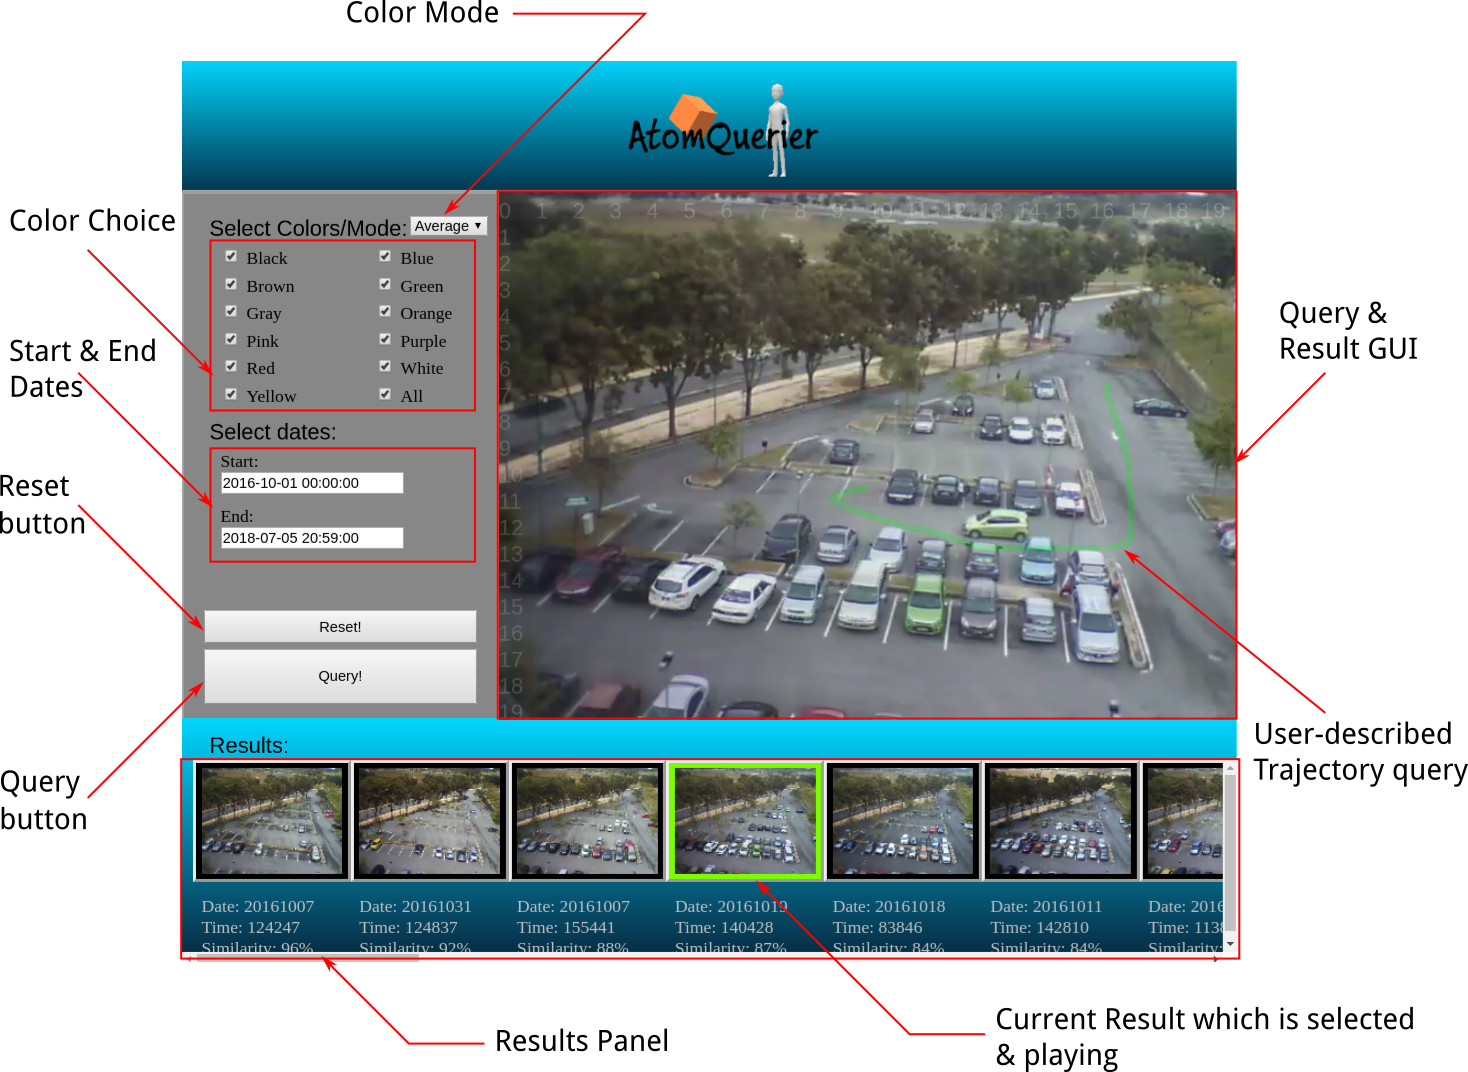
\includegraphics[width=.9\textwidth]{image/retrievalTwo/VISERinterface2.png}
\caption{Search Interface for \versionTwoRet}
\label{fig:versionTwoInterface}
\end{figure}

\subsection{Metrics, Scoring System and Experimental Methodology}

The following subsections describes the scoring system, metrics as well as the evaluation process of the proposed method described in Section \ref{section:versionTwo}. Given that the main objective of the proposed retrieval engine is to provide users with results which closely resemble the given query in a sorted manner such that results which are more relevant should appear higher in the rank. The performance of the proposed method was measured using the \textit{Precision@K} and normalised Discounted Cumulative Gain (\textit{nDCG}) metrics.

The \textit{Precision@K} metric is used to identify the number of retrieved results which are relevant to the user while the \textit{nDCG} metrics is used to measure how well the retrieval engine's results are ordered for the end users. The idea behind \textit{DCG} is that results that are highly relevant are more useful when it appears higher in rank, users would not need to go through too many results before finding a suitable and relevant result. The other side of the coin is true as well, relevant documents which appears lower in the rank should be penalised, hence the discount in its gain.

In order to evaluate the performance of the proposed method, the evaluation of both the trajectory and colour terms were separated. The separation of evaluations allows further understanding on how to improve the retrieval engine as a whole. A group of volunteers were introduced to the retrieval engine along with it's features and a sample use case was demonstrated, then, the volunteers were given full control to draw any query they were interested in. Next with the results from the retrieval engine, the volunteers were tasked to provide feedback by rating each result with a scale of 1 to 5, with 5 being a result that closely resembles the input query.

The volunteers were given full control of the input query $\mathbb{P}$ as it closely resembles real world scenarios. With that in consideration, it is not feasible to obtain the ground truth annotation for each of those queries within the one month data time frame, without which the recall rate can not be measured for this retrieval engine.
While the \textit{Precision@K} metrics is a commonly used metric for retrieval system, the main disadvantage of this metric is that the evaluation process is done in a coarse manner as it only provides a binary evaluation of whether or not a particular result is relevant to the query. On the other hand, the \textit{DCG} metric is able to provide a more granular evaluation of the proposed method as the results are evaluated based on its ordered rank along with the relevancy of the result. Figure \ref{fig:dcgGain} illustrates the decreasing gain value of each result as the ranking of the result increases.

\begin{figure}[!ht]
\centering
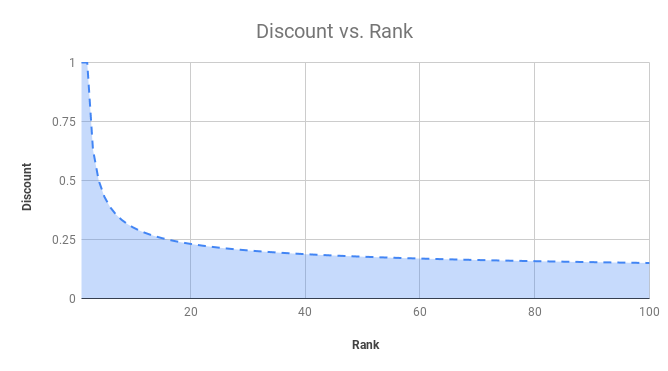
\includegraphics[width=0.9\textwidth]{image/retrievalTwo/discountvsrank.png}
\caption{The Discounted Gain Decreases Exponentially as Rank Increases}
\label{fig:dcgGain}       % Give a unique label
\end{figure}

\begin{equation}
\label{eq:DCGk}
DCG_p = \sum_{p=1}^k\frac{REL_{p}}{\log_2 (\max (p,2))}
\end{equation}

% $DCG@K = \sum_{i=i}^K\frac{REL_{i}}{\log_2 (\max (i,2))}$

Since the Discounted Cumulative Gain metric produces an unbounded value ([0, $\infty$) range), it is not suitable for use when averaging across multiple independent queries. In order to make use of the \textit{DCG} metric, it is converted into the \textit{nDCG} metrics using Equation \ref{eq:nDCG} where the values are now bounded within a [0, 1] range.
\begin{align}
\label{eq:nDCG}
\textit{nDCG}_P = \frac{DCG_P}{IDCG_P}
\end{align}
where:

\hspace{2em} $IDCG_P$ is the ideal DCG score at Rank P in the ideal ranking order.

The following subsections provides in-depth details on the experimental methodology which were designed for the evaluation of the retrieval engine's ability to retrieve both the vehicle trajectory as well as vehicle colours.


\subsubsection{Vehicle Trajectory}
 The volunteers were given full control of the user interface and asked to draw at least 1 trajectory as an input query. Upon performing the query, the volunteers were asked to rate each of the resulting trajectory video shot with a scale from 1 to 5, where 1 signifies the least relevant, and 5 being the most relevant.

 Each input query would return at least 25 results which were ordered randomly, this was intentionally done to prevent the volunteers from having any pre-conceived idea of how the results should be ordered which would affect the way each retrieved results is judged. By removing the biasness, the volunteers were able to provide a fair and sound evaluation towards each result, hence increasing the credibility of the overall results.



\subsubsection{Vehicle colour \& colour Mode}
\label{subsec:vehColor}
A list with a total of 330 video snippets (30 video snippets for each of the 11 common colours) were presented to the volunteers. These 30 video snippets from each colours were selected using the top 30 results in the database which contained the highest probability for each of the colours. The volunteers were then asked to determine the relevance of the colour term to that particular vehicle for each of the 330 video snippets with the same scale from 1 to 5.

In order to thoroughly evaluate the performance of the colour semantic extraction process which was introduced in Section \ref{section:versiontwoColor}, three other colour modes were included in the evaluation process. These colour modes are variations on how the colour terms are extracted using different colour space and distance metrics. These variations are listed in Table \ref{table:ColorVariation}.

\begin{table}[!ht]\centering
\begin{tabular}{|c|l|}
\hline
Colour Mode & Distance Metrics \\
\hline
LUV &
\begin{tabular}{lcl}
\\
$\mean{r}$ &  $=$  & $\frac{C_{1R} + C_{2R}}{2}$\\
$\Delta R$ & $=$ & $C_{1R} - C_{2R}$\\
$\Delta G$ & $=$ & $C_{1G} - C_{2G}$\\
$\Delta B$ & $=$ & $C_{1B} - C_{2B}$\\
\\
$\Delta Colour_{LUV}$ & $=$ &$\sqrt{(2 + \frac{\mean{r}}{256}) \times \Delta R^{2} + 4 \times \Delta G^{2} + (2 + \frac{255 - \mean{r}}{256}) \times \Delta B^{2}}$
\\
\hspace{4em}& & \\
\end{tabular}\\
\hline
HSV &
\begin{tabular}{lcl}
\\
\multicolumn{3}{c}{(As introduced in Section \ref{section:versionOneColorExtract})}
\\

$\Delta{Hue}$ & $=$ & $\min\{ \mid GT_{hue} - Colour_{hue} \mid,  180^{\circ} - \mid GT_{hue} - Colour_{hue} \mid  \}$ \\
$\Delta  Saturation$ & $=$ & $GT_{saturation} - Colour_{saturation}$ \\
$\Delta  Value$ &  $=$ & $GT_{Value} - Colour_{Value}$ \\
\\
$\Delta Colour_{HSV}$ & $=$ & $\sqrt{\Delta{Hue}^{2} + \Delta{Sat}^{2}  + \Delta{Val}^{2} }$
\\
\hspace{4em}& & \\
\end{tabular}\\
\hline
Lab &
\begin{tabular}{lcl}
\\
$\Delta L$ & $=$ & $C_{1L} - C_{2L}$\\
$\Delta a$ & $=$ & $C_{1a} - C_{2a}$\\
$\Delta b$ & $=$ & $C_{1b} - C_{2b}$\\
\\
$\Delta{Colour_{Lab}}$ & $=$ & $\sqrt{\Delta{L}^{2} + \Delta{a}^{2}  + \Delta{b}^{2} }$
\\
\hspace{5em}& & \\
\end{tabular}\\
\hline
Average &
\begin{tabular}{lcl}
\\
$\Delta{Colour_{Average}}$ & $=$ & $\frac{\Delta{Colour_{LUV}} + \Delta{Colour_{HSV}} + \Delta{Colour_{Lab}}}{3}$
\\
\hspace{4em}& & \\
\end{tabular}\\
\hline
\end{tabular}
\caption{Variation of colour Distance Metrics Used}
\label{table:ColorVariation}
\end{table}


\subsection{Results and Analysis}

The results of both components (Vehicle Trajectory \& Vehicle Colour) are recorded in this section. As the results were evaluated using a scale from 1 to 5, these results were converted using a binary evaluation (True(1) / False(0)). This is done to enable to evaluation using the \textit{Precision@K} metrics. Here, results scoring with an average of 3 and above are considered relevant to the query. Each relevant (True(1)) result \textit{(n)} will then contribute to the \textit{Precision@K} score (see Equation \ref{eq:p@k}).
 \begin{equation}
\label{eq:p@k}
Precision@K =  \frac{\sum_{n=1}^K \begin{cases}1 \rightarrow True, & AvgScore(Result_n)\geq 3\\0 \rightarrow False, & AvgScore(Result_n)< 3 \end{cases}} {K}
\end{equation}

\subsubsection{Vehicle Trajectory}
A total of eleven trajectories were drawn by six volunteers who were given full liberty on how each was drawn. Figure \ref{fig:versionTwoTrajquery} shows a compilation of these trajectories overlaid over the car park scene, these trajectories covered a majority of the scene while showing a good mixture of different queries.
While some of the queries exceeded the tracking area of the tracker, the retrieval engine managed to retrieved results which has the closest resemblance to the given queries. As mentioned, the performance of the retrieval engine was measured using \textit{Precision@K} along with the \textit{normalised Discounted Cumulative Gain} (\textit{nDCG}) metrics.

\begin{figure}[!t]
  \centering
    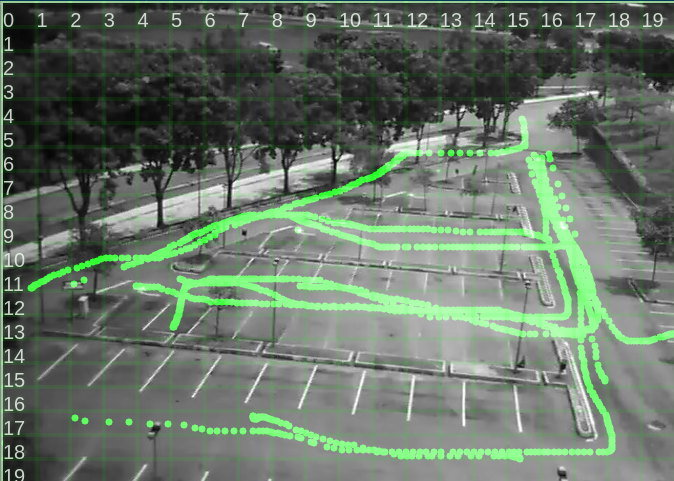
\includegraphics[width=0.8\linewidth]{image/retrievalTwo/trajquery.png}
  \caption{Compilation of Trajectory Queries Provided by Volunteers}
  \label{fig:versionTwoTrajquery}
\end{figure}

Even though the errors from the tracker\cite{lim2017} cascaded into database, results due to tracker error was not removed to provide a general idea of the retrieval engine's performance when working with trackers which are currently available. First, the \textit{Precision@K} of the retrieval engine was measured and recorded, Figure \ref{fig:versionTwoPreAtK} contains the plot of the average \textit{Precision@K} result. The result shows that the retrieval engine managed to retrieve video shots which were relatively relevant to the user's query with an average precision of 76\%. The \textit{Precision@K} results shows a steady decline in its precision as the K (number of results) increases, this was an expected outcome as it is common in a regular retrieval engine.

\begin{figure}[!ht]
  \centering
    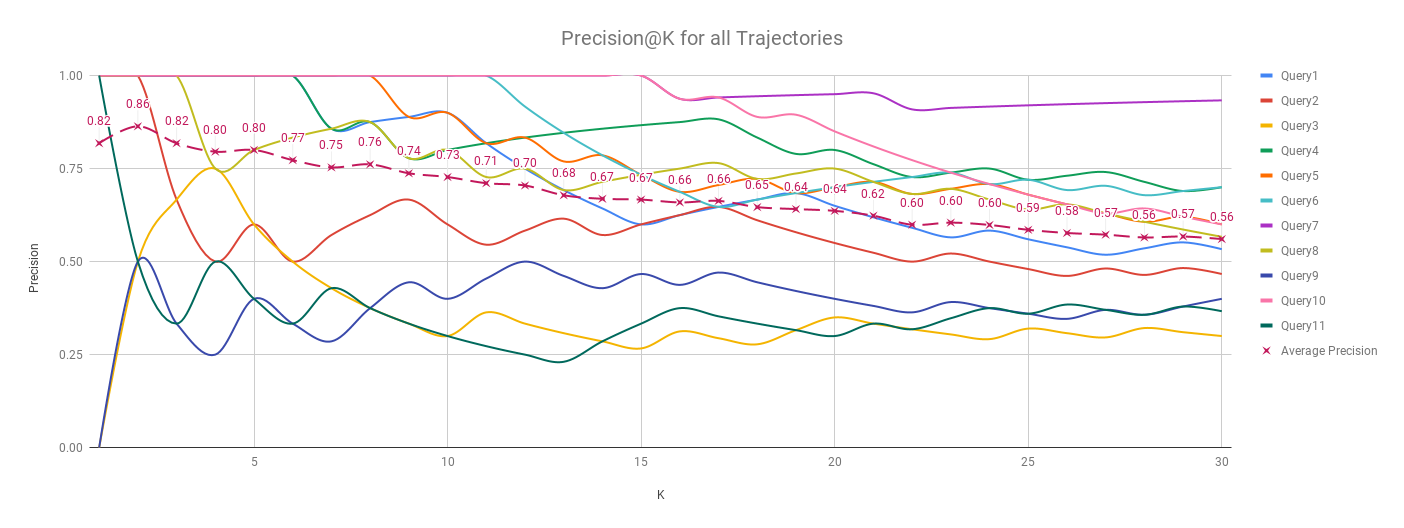
\includegraphics[width=\linewidth]{image/retrievalTwo/p@k.png}
  \caption{Precision at K for All Trajectory Queries}
  \label{fig:versionTwoPreAtK}
\end{figure}

Next, in order to determine the retrieval engine's overall performance in regards to how the results were ordered, the average \textit{nDCG} score for all eleven trajectory queries were measured and plotted in Figure \ref{fig:ndcgWithError}. As a whole, the average \textit{nDCG} score lies along the 83\% region. This means that the results were 83\% of the time ordered in the best possible manner. As the number of retrieved results were evaluated, the \textit{nDCG} score shows an increase.
While this is not desirable, this behaviour was expected. A good retrieval engine would strive to provide the best results in the best order if possible.

\begin{figure}[!ht]
  \centering
    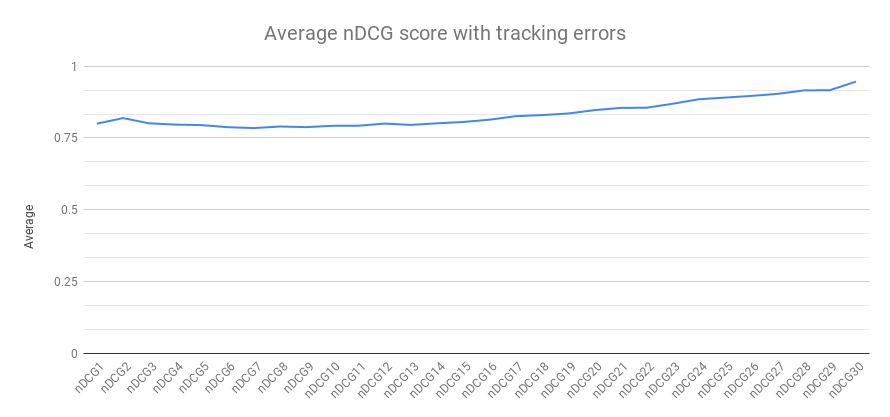
\includegraphics[width=0.9\linewidth]{image/retrievalTwo/averageNDCG.png}
  \caption{Average Normalised Discounted Cumulative Gain Score}
  \label{fig:ndcgWithError}
\end{figure}

To further break down the evaluation process of the retrieval engine's performance, as per the previous retrieval model's evaluation, the trajectory queries were also divided into two categories: \textit{simple} and \textit{complex} trajectories. \textit{Simple} trajectories refers to trajectories that moves in a single direction without any turning (such as a straight line) while \textit{complex} trajectories refers to movements which consist of more than one turning. Table \ref{table:versionTwoComplexSimple} shows the category of each query while the \textit{Precision@K} results are plotted in Figure \ref{fig:versionTwoPatKAll}.

For simple trajectories, the Precision@K scores a high 100\% at the beginning and slowly decrease to around 68\% as the number of retrieved results (K) were reviewed. All the simple queries shows rather consistent results which are as expected. As for complex trajectories, the precision at k=1 started at 67\% and dropped further to 46\% at the end of 30 results. Even though Query 6 and Query 9 belongs in the complex trajectory category, the first 10 results shows rather high precision. However, the results from the other complex trajectory did not perform as well as Query 6 and Query 9. The results of those query started strong in the early K, but dropped significantly when K was 3 and above. The overall Precision@K results shows a rather expected behaviour where the precision would be high in the early K region, and would slowly decrease as K increases.

% Please add the following required packages to your document preamble:
% \usepackage{multirow}
\begin{table}[!ht] \centering
\begin{tabular}{|c|l|}
\hline
\multicolumn{1}{|l|}{\textbf{Trajectory Category}} & \textbf{Query Number} \\ \hline
\multirow{5}{*}{Simple} & Query 4 \\ \cline{2-2}
 & Query 5 \\ \cline{2-2}
 & Query 7 \\ \cline{2-2}
 & Query 8 \\ \cline{2-2}
 & Query 10 \\ \hline
\multirow{6}{*}{Complex} & Query 1 \\ \cline{2-2}
 & Query 2 \\ \cline{2-2}
 & Query 3 \\ \cline{2-2}
 & Query 6 \\ \cline{2-2}
 & Query 9 \\ \cline{2-2}
 & Query 11 \\ \hline
\end{tabular}
\caption{Queries and the Corresponding Trajectory Type}
\label{table:versionTwoComplexSimple}
\end{table}

As a whole, both \textit{simple} and \textit{complex} queries shows reasonably good performance in terms of its precision, however, when evaluated individually, the \textit{complex} queries shows poorer results. Next, the \textit{nDCG} score of both the \textit{simple} and \textit{complex} trajectory queries were evaluated and plotted in Figure \ref{fig:versionTwoNDCG}(a) and Figure \ref{fig:versionTwoNDCG}(b) respectively.


\begin{figure}[htb!]
  \centering
\begin{tabular}{c}
 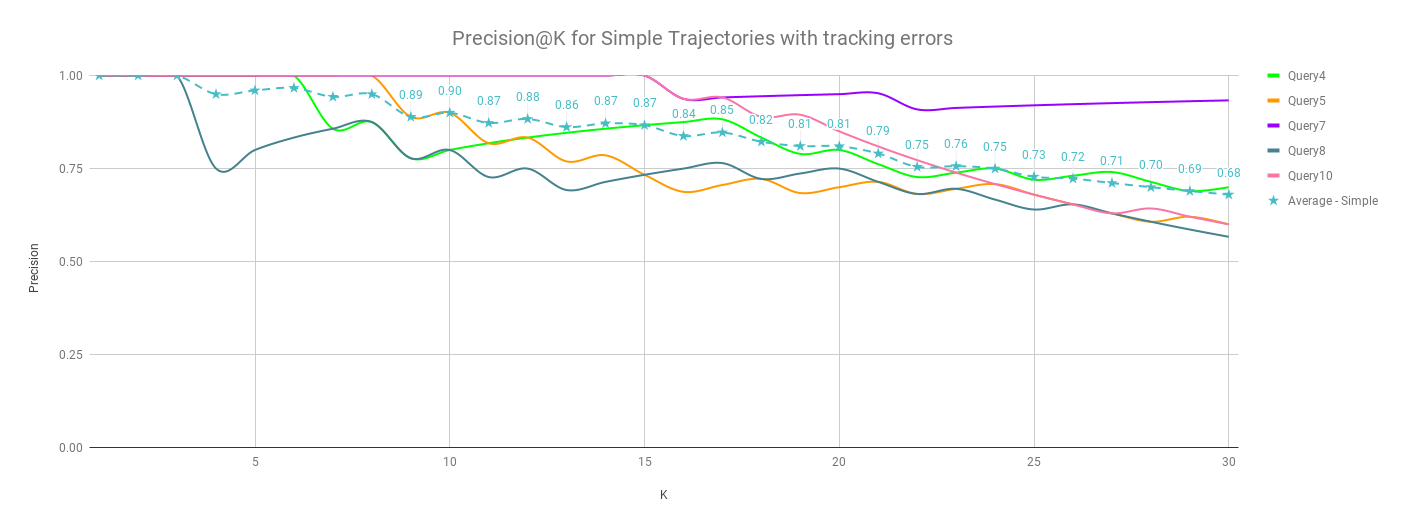
\includegraphics[width=0.9\linewidth]{image/retrievalTwo/p@k_simple.png}\\
 (a) \textit{Precision@K} for Simple Trajectories \\
 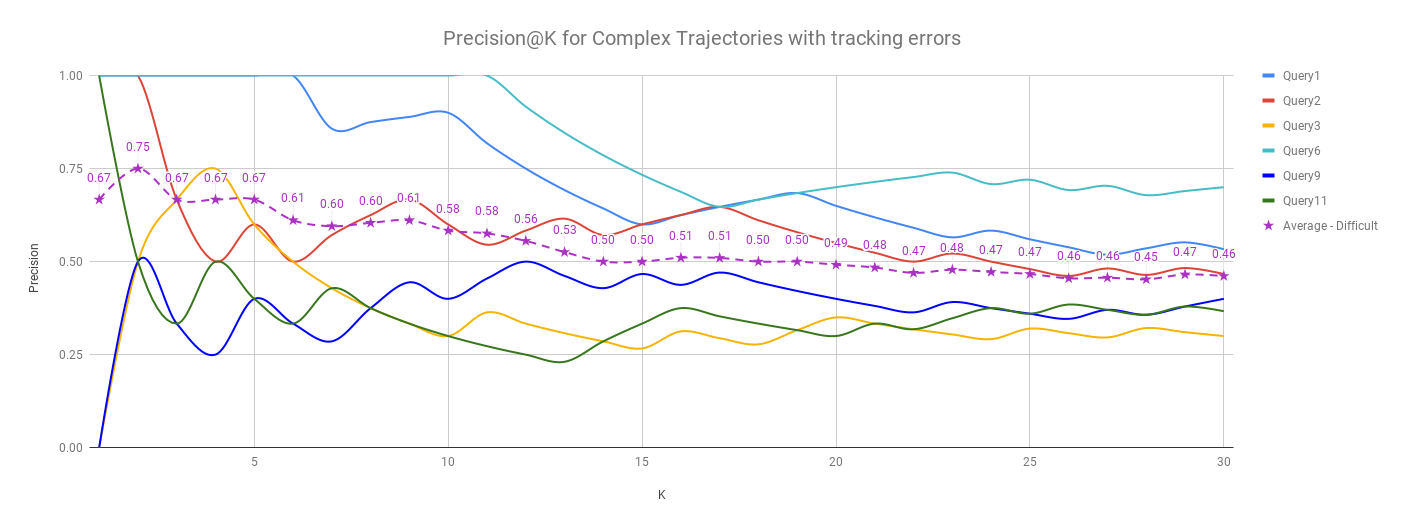
\includegraphics[width=0.9\linewidth]{image/retrievalTwo/p@k_complex.png} \\
 (b) \textit{Precision@K} for Complex Trajectories
\end{tabular}
\caption{\textit{Precision@K} for Simple and Complex Trajectories Queries} \label{fig:versionTwoPatKAll}
\end{figure}


\begin{figure}[htb!]
  \centering
\begin{tabular}{c}
 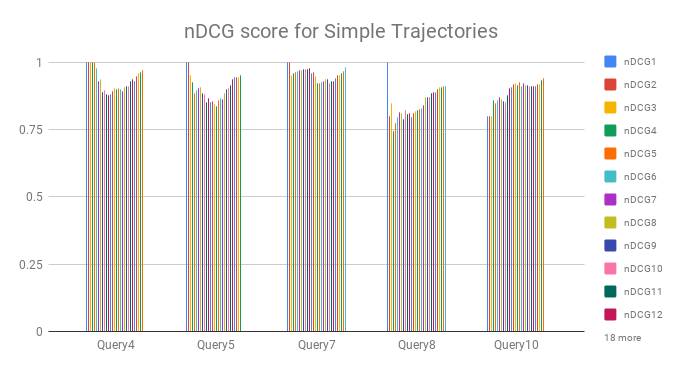
\includegraphics[width=0.9\linewidth]{image/retrievalTwo/ndcgSimple.png}\\
 (a) \textit{nDCG} for Simple Trajectories \\
 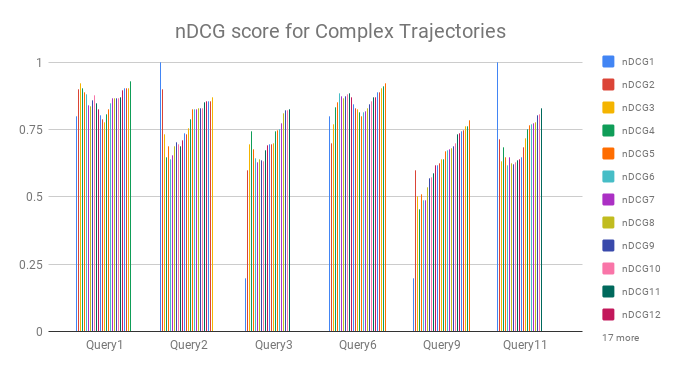
\includegraphics[width=0.9\linewidth]{image/retrievalTwo/ndcgComplex.png} \\
 (b) \textit{nDCG} for Complex Trajectories
\end{tabular}
\caption{Normalised Discounted Cumulative Gain for Simple and Complex Trajectories Queries} \label{fig:versionTwoNDCG}
\end{figure}

The difference between the simple and complex trajectories are rather distinct. The overall nDCG score for the queries of simple trajectories were rather high in the 91\% region while the nDCG score for queries related to complex trajectories were in the 75\% region. The results here shows that the retrieval engine had an easier time sorting simple trajectories in the best ranking order while having some difficulty when organising the complex trajectories using the $D_{chamfer}$ metrics. Even though the overall results are relatively good, the implementation of Chamfer Distance in the proposed method is not without its faults. Observation of the results shows that chamfer distance performs poorly when (i) a trajectory is compared against a much shorter trajectory that intersects at a particular point or (ii) two trajectories turning into 2 different junctions. In both examples, the obtained $D_{chamfer}$ shows relatively low score that could result in those shots being retrieved, these examples can be found in Figure  \ref{fig:chamferDisadvantage}.

\begin{figure}[htb!]
  \centering
\begin{tabular}{cc }
 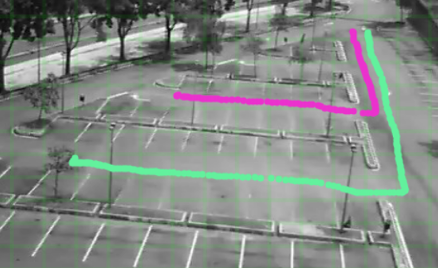
\includegraphics[width=0.45\linewidth]{image/retrievalTwo/chamferDisadv2.png} &
 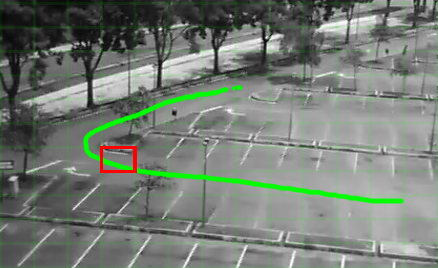
\includegraphics[width=0.45\linewidth]{image/retrievalTwo/chamferDisadv1.png} \\
 (a) Two trajectories with similar shape &
 (b) Trajectory intersecting with a point \\
\end{tabular}
\caption{Disadvantages of Chamfer Distance} \label{fig:chamferDisadvantage}
\end{figure}



\cc{for the analysis, include a "heatmap" of the versionone vs versiontwo for the evaluation of results} \\
\cc{why the colour metric selected worked best (higher difference btween each term)}


In a nutshell, despite the flaws of Chamfer Distance, the implementation of $D_{chamfer}$ in the retrieval engine provided relatively good results (Average \textit{Precision@K} = 76\%) that were sorted in an organised and useful manner (\textit{nDCG} score = 83\%). The use of Chamfer Distance can be extended to other datasets of similar properties.

\subsubsection{Vehicle Colour \& Colour Mode}
\label{subsec:vehiclecolourchamferdistanceexperiment}

As mentioned in Section \ref{subsec:vehColor}, a total of 330 video snippets were extracted from the top 30 results of each colour modes were extracted. As four colour modes were tested, the six volunteer were split into groups of three and they were given two sets of data to evaluate.
The results of the average \textit{Precision@K} metric for each of the colour modes were tabulated in Figure \ref{fig:colorspace_score} while Table \ref{tab:avg@k} shows a high level overview of the results across K = 1 to 30. Similar to the evaluation process of the vehicle trajectories, this time, the volunteers were asked to determine the relevance of the colour term to that particular vehicle for each of the video snippets with a scale of 1 to 5.

\begin{table}[!t]
	\centering
	\caption{Average Precision @ K for Each Colour Metrics}
	\label{tab:avg@k}
\begin{tabular}{c||c|c|c|c|c|c|c|c|c|c}
K & 1 & 2 & 3 & 4 & 5 & 10 & 15 & 20 & 25 & 30  \\ \hline \hline
\rowcolor{yellow} LUV  & 0.91 & 0.91 & 0.91 & 0.86 & 0.85 & 0.69 & 0.62 & 0.60 & 0.63 & 0.60 \\
Lab  & 0.27 & 0.27 & 0.27 & 0.25 & 0.24 & 0.24 & 0.24 & 0.23 & 0.22 & 0.22 \\
HSV & 0.27 & 0.36 & 0.30 & 0.27 & 0.29 & 0.25 & 0.25 & 0.23 & 0.21 & 0.21 \\
Avg & 0.09 & 0.18 & 0.15 & 0.16 & 0.16 & 0.18 & 0.18 & 0.20 & 0.23 & 0.23 \\
\end{tabular}
\end{table}


\begin{figure}[htb!]
  \centering
\begin{tabular}{cc}
 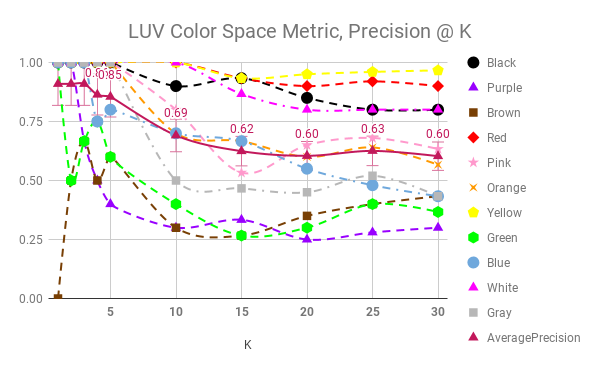
\includegraphics[width=0.5\linewidth]{image/new/luv@k.png} &
 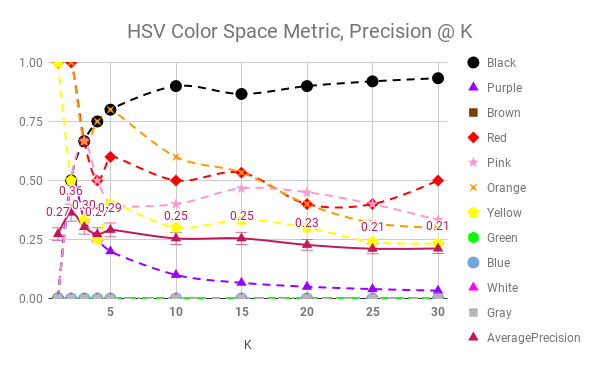
\includegraphics[width=0.5\linewidth]{image/new/hsv@k.png}\\
 (a) LUV colour Mode &
 (b) HSV colour Mode \\
 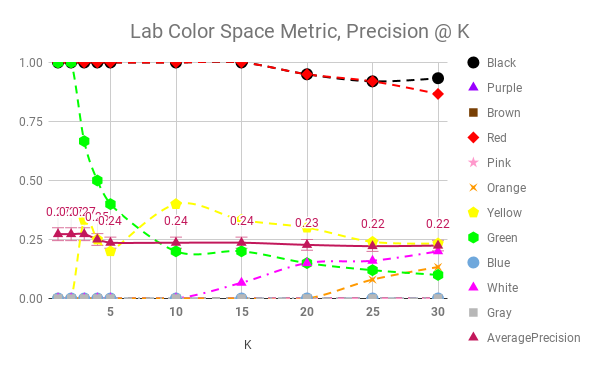
\includegraphics[width=0.5\linewidth]{image/new/lab@k.png} &
 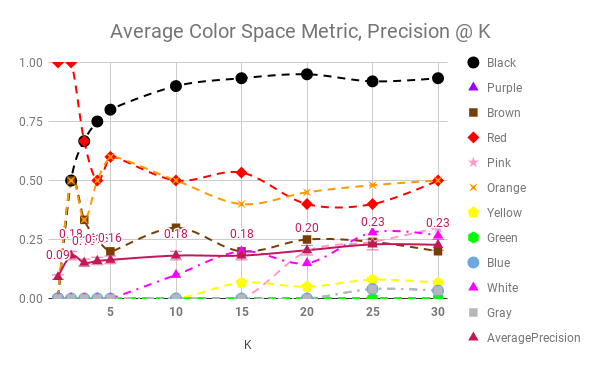
\includegraphics[width=0.5\linewidth]{image/new/avg@k.png} \\
 (c) Lab colour Mode&
 (d) Average colour Mode \\
\end{tabular}
\caption{\textit{Precision@K} for Each colour Mode} \label{fig:colorspace_score}
\end{figure}

The \textit{Precision@K} results of the LUV colour mode showed the best results among the other colour modes used to extract the colour term. The average precision at K=1 is at an amazing 91\%, however, by the time K=10, the precision has dropped to an average precision of 69\% and gradually drops to 60\% when K reached 30. The colours Yellow, Red, Black, and White showed rather consistent results throughout the experiment while colours like Purple, Green and Brown fared rather poorly. This was likely because there were not many cars which were highly saturated in those colours.

When comparing with the other colour modes, Black colour tend to provide consistent results throughout the entire experiment. The average precision for the HSV and Lab colour modes was staggering around the 25\% region. It is also observed that the retrieval of Red and Black colour vehicles perform significantly well in the Lab colour space when compared to the other colours, the average precision of these two colours are in the 90\% vicinity.

During the phase of preparing the experimental methodology, the average colour mode was designed with the goal of maximising the strength of each colour modes while averaging out the weaknesses. However, based on the conducted experiment, it was surprising to see the underwhelming performance of the HSV and Lab colour mode. Hence, the average colour mode also took a dive in terms of the precision. However, this colour mode did live up to its expectation in maximising the strengths of each colour modes. Based on the results tabulated, the precision when retrieving Black colour vehicles was rather well except for the initial precision during the early K region which were unexpected.

To further analyse the performance of the colour modes used, the confusion matrix of each colour mode used is plotted in Figure \ref{fig:colorspace_Confuscore} using 30 results for each colour term (with a total of 330 results for each colour space). The X-axis represents the Actual Colour, while the Y-axis represents the Predicted Colour. The colours in the confusion matrix were arranged in the following order: Black, Purple, Brown, Red, Pink, Orange, Yellow, Green, Blue, White, Gray. This colours were ordered based on its perceived similarity in terms of saturation and brightness. In the figure, the X-axis also contains an additional row which indicates numbers of results which were due to tracking error in the initial tracking  phase.

\begin{figure}[htb!]
  \centering
\begin{tabular}{cc}
 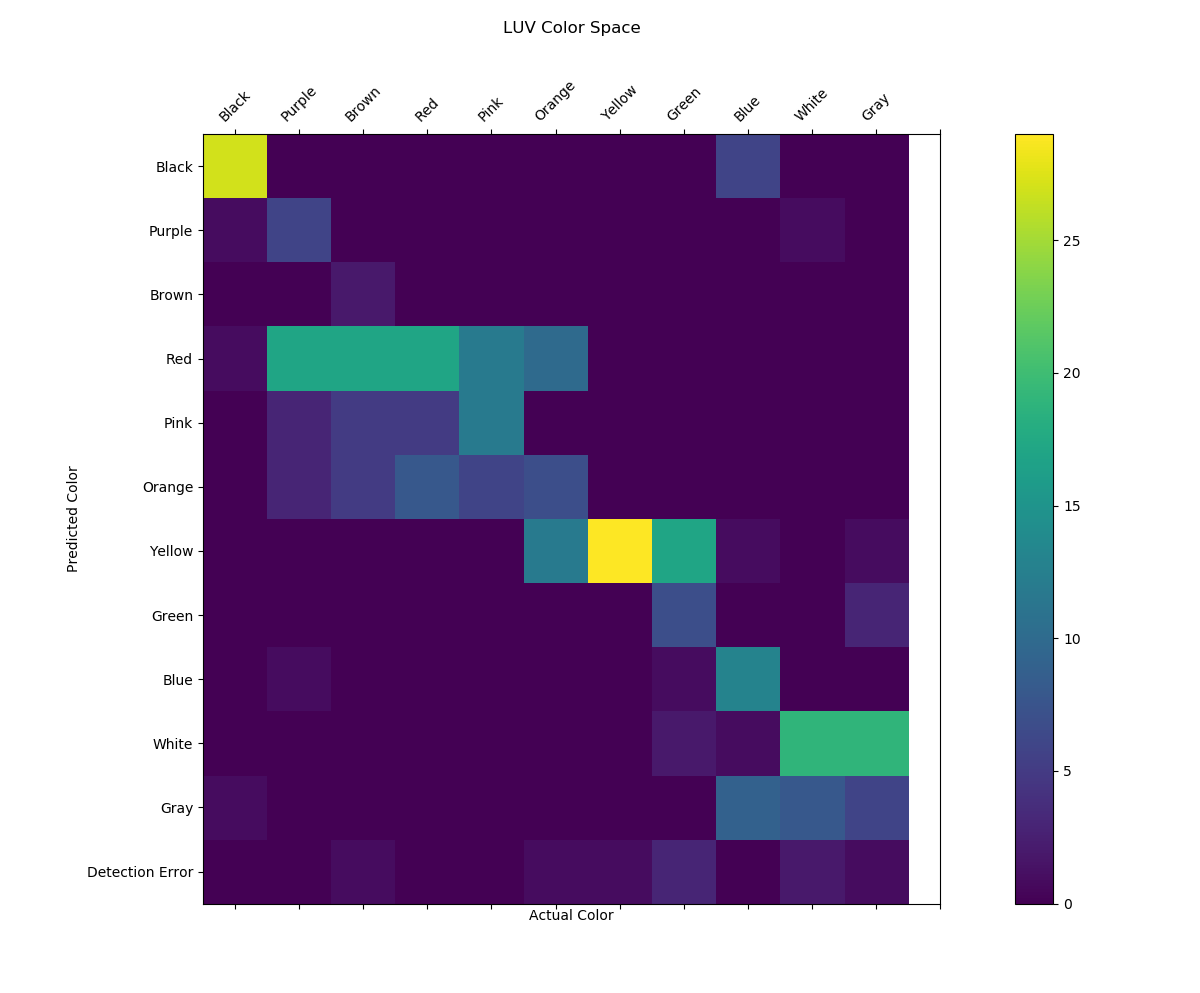
\includegraphics[width=0.4\linewidth]{image/retrievalTwo/luvCM.png} &
  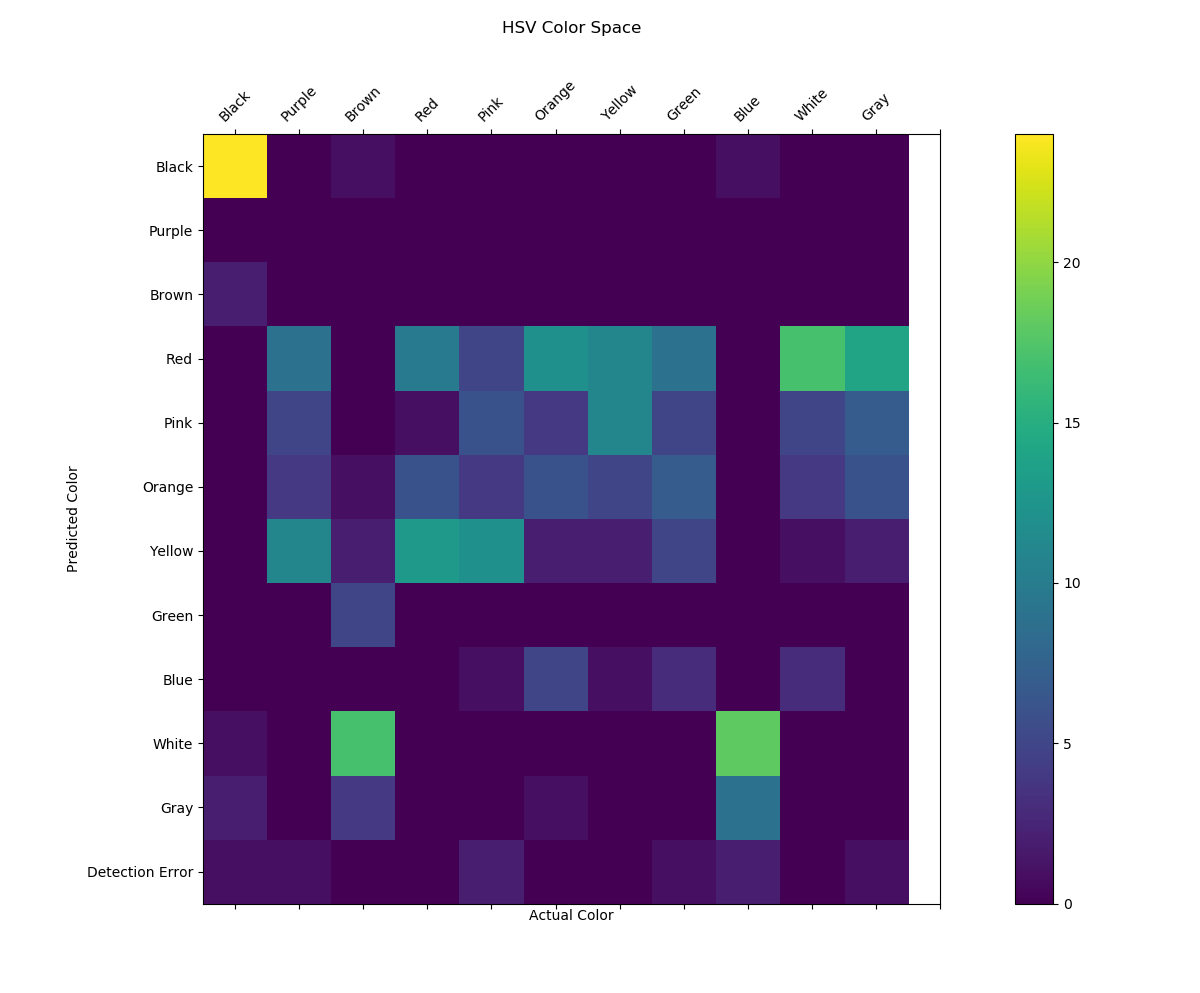
\includegraphics[width=0.4\linewidth]{image/retrievalTwo/hsvCM.png} \\
 (a) LUV colour Mode & (b) HSV colour Mode \\
 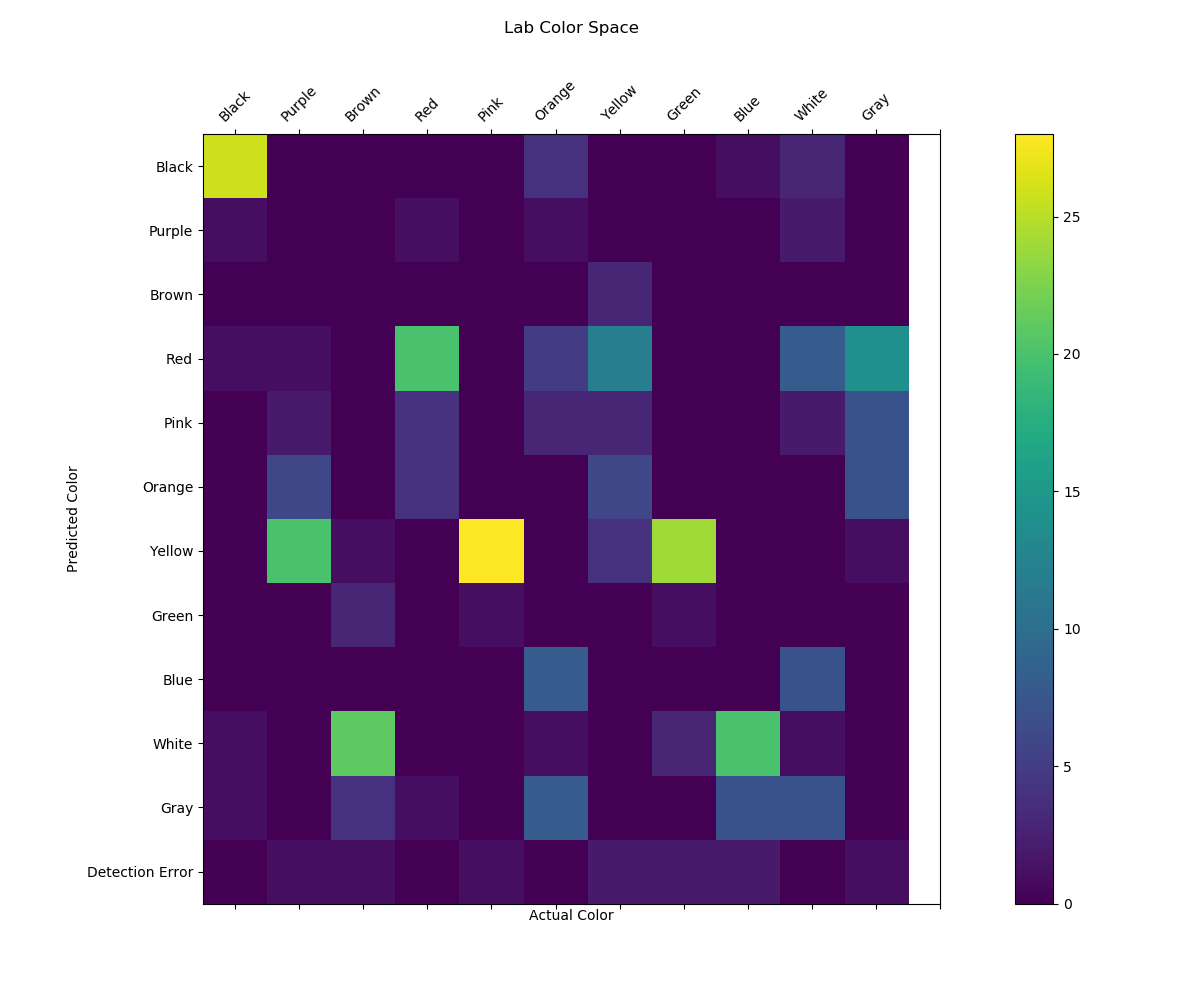
\includegraphics[width=0.4\linewidth]{image/retrievalTwo/labCM.png} &
 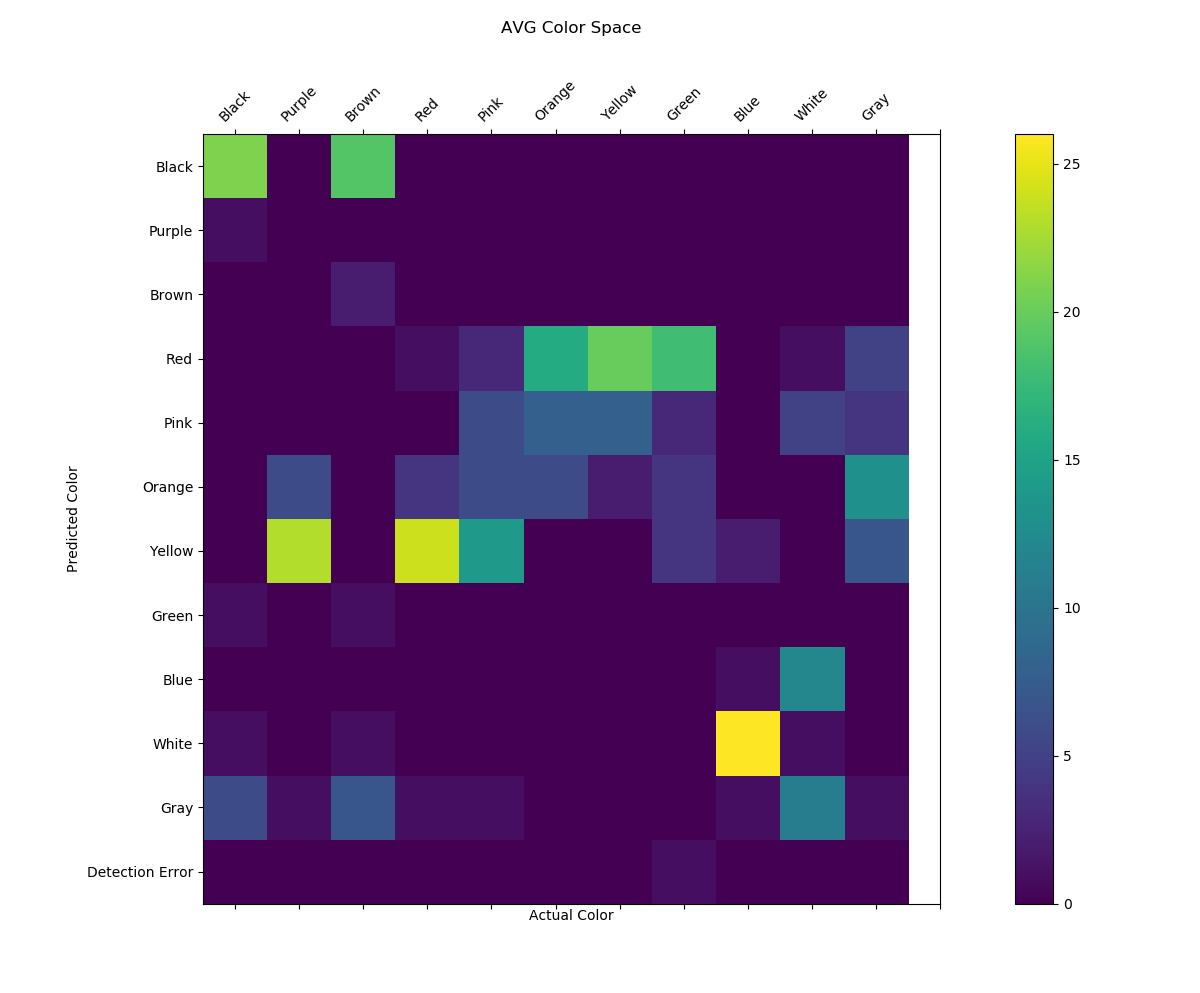
\includegraphics[width=0.4\linewidth]{image/retrievalTwo/avgCM.png} \\
(c) Lab colour Mode & (d) Average colour Mode \\
\end{tabular}
\caption{Comparison Between the colour Modes Using Confusion Matrix} \label{fig:colorspace_Confuscore}
\end{figure}

Upon further inspection of the tabulated confusion matrices, the results shows similar output when compared with the \textit{Precision@K} results recorded from the volunteers via the scoring method. Both the results tallies in their finding that the low cost LUV colour mode proposed by Riemersma\cite{riemersma} outperforms the other colour modes. The Euclidean distance metrics used in the HSV colour mode to extract the colour terms performed the worst with not much variation in the results for each colour. On the other hand, the Lab colour mode's results showed a considered amount of accuracy for strongly distinct colours such as Red and Black but fails to differentiate the rest as visualised in Figure \ref{fig:colorspace_Confuscore}(C).

Since the LUV colour mode's \textit{Precision@K} metrics outperformed the rest with a precision of 85\% at k=5, while the other colour modes barely reached the 30\% mark, only the normalised Discounted Cumulative Gain (\textit{nDCG}) for the LUV colour mode results were measured and plotted to understand the performance of the retrieval engine in terms of how well the results were sorted. Since the HSV, Lab and Average colour space metrics did not perform well, the nDCG metric was not measured as the order of the results does not represent the actual performance of the retrieval engine. The Discounted Cumulative Gain result was also visualised using Figure \ref{fig:colorndcg}.

The Bar chart is used to represent the number of results the user has to view in order to find a relevant document, hence a chart where the results consistently stays at the high 80-100\% area shows that the ranking of the results were done in one of the best ways possible. The Radar chart on the other hand, represents the overall performance of a particular colour over the number of results the user has to view in order to find a relevant document. Both of the charts clearly visualise that most colours were retrieved accurately and sorted in the a relatively good order with an astounding performance of high 80-90\% except for Brown and Green colour where the retrieval engine's performance only reach the best at the end of 30 results.


\begin{figure}[htb!]
  \centering
\begin{tabular}{c}
 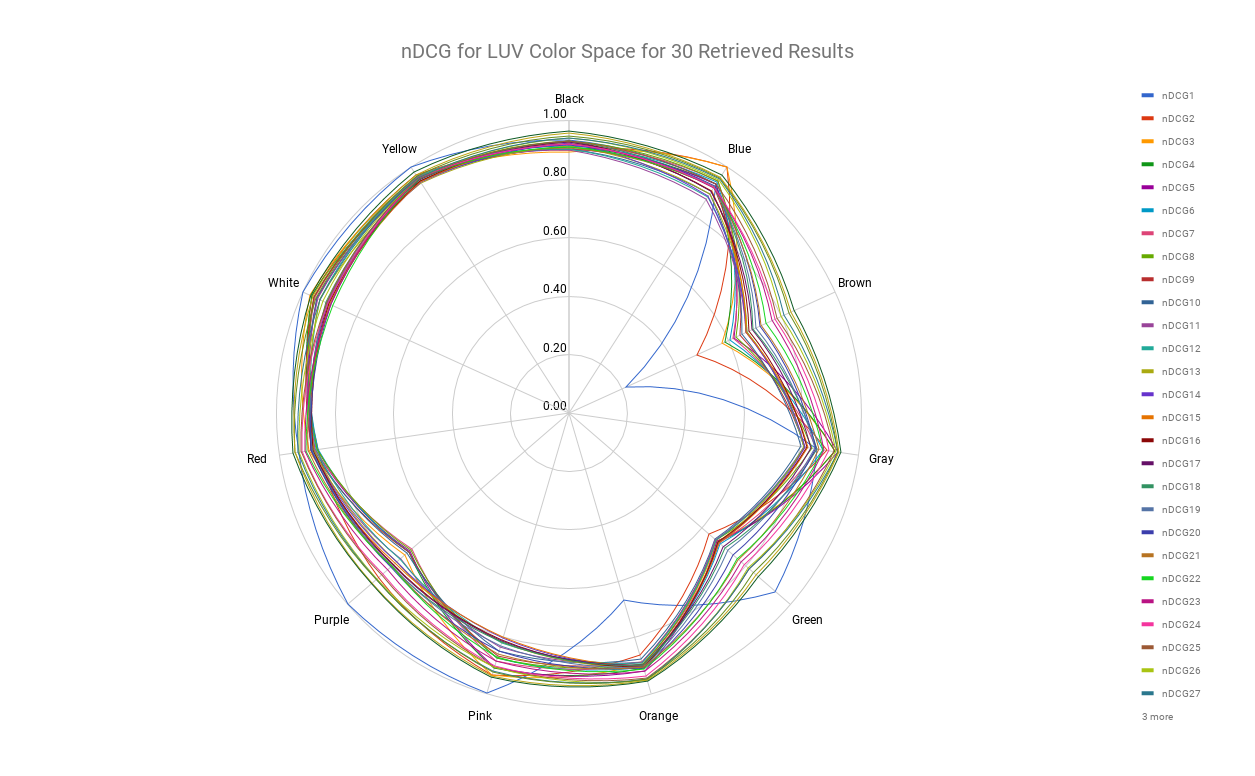
\includegraphics[width=0.9\linewidth]{image/retrievalTwo/radar_ndcg_luv.png}\\
 (a) \textit{nDCG} visualised in Radar Chart \\
  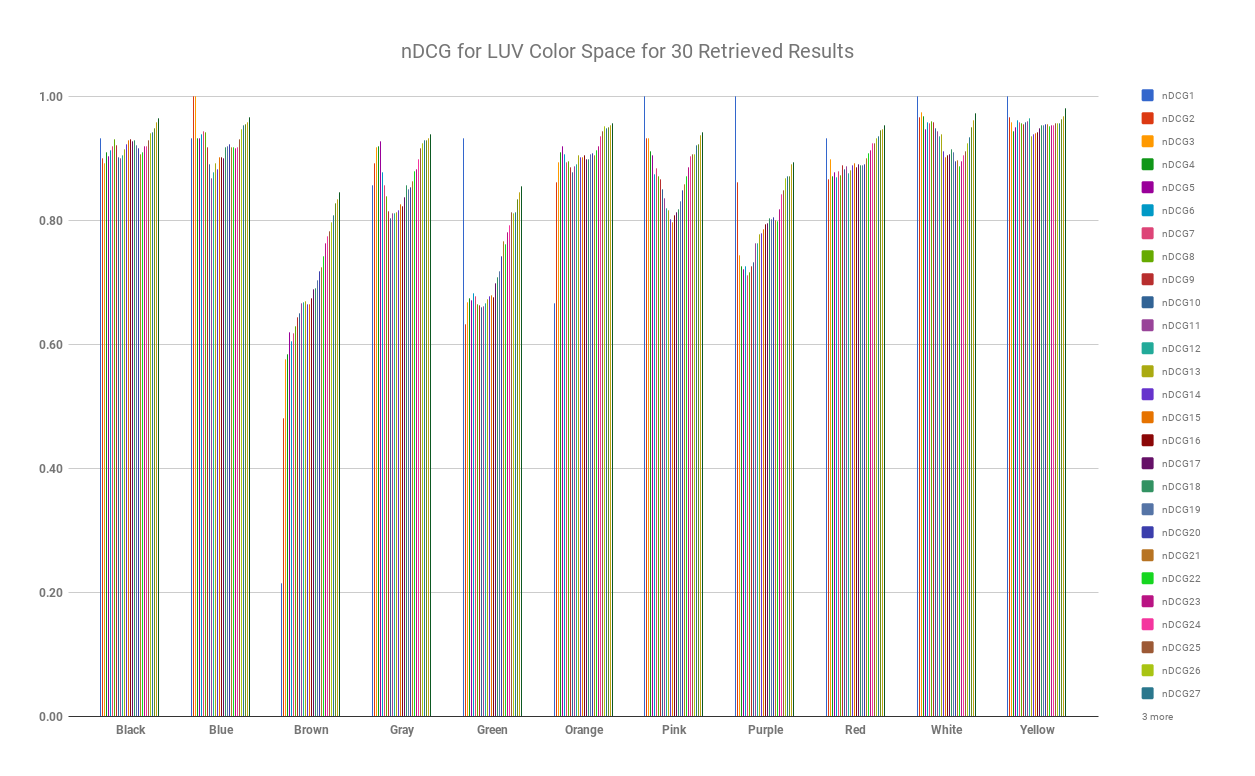
\includegraphics[width=0.9\linewidth]{image/retrievalTwo/bar_ndcg_luv.png}\\
 (b) \textit{nDCG} visualised in Bar Chart \\
\end{tabular}
\caption{\textit{nDCG} of the LUV Colour Mode using Radar and Bar Chart} \label{fig:colorndcg}
\end{figure}


\begin{table}[ht!]
	\centering
	\caption{Normalised Discounted Cumulative Gain (nDCG) for the LUV colour metrics}
	\label{tab:dcgColor}
\resizebox{\textwidth}{!}{
\begin{tabular}{c||c|c|c|c|c|c|c|c|c|c|c}
& Black & Blue & Brown & Gray & Green & Orange & Pink & Purple & Red & White & Yellow \\ \hline \hline
\textit{nDCG1} & 0.93 & 0.93 & 0.21 & 0.86 & 0.93 & 0.67 & 1.00 & 1.00 & 0.93 & 1.00 & 1.00 \\
\textit{nDCG2} & 0.90 & 1.00 & 0.48 & 0.89 & 0.63 & 0.86 & 0.93 & 0.86 & 0.87 & 0.97 & 0.97 \\
\textit{nDCG3} & 0.89 & 1.00 & 0.58 & 0.92 & 0.67 & 0.89 & 0.93 & 0.74 & 0.90 & 0.97 & 0.96 \\
\textit{nDCG4} & 0.91 & 0.93 & 0.58 & 0.92 & 0.68 & 0.91 & 0.91 & 0.73 & 0.87 & 0.97 & 0.94 \\
\textit{nDCG5} & 0.90 & 0.93 & 0.62 & 0.93 & 0.67 & 0.92 & 0.90 & 0.72 & 0.88 & 0.95 & 0.95 \\
\textit{nDCG6} & 0.91 & 0.94 & 0.60 & 0.88 & 0.68 & 0.91 & 0.87 & 0.73 & 0.87 & 0.96 & 0.96 \\
\textit{nDCG7} & 0.92 & 0.94 & 0.62 & 0.86 & 0.68 & 0.89 & 0.88 & 0.71 & 0.88 & 0.96 & 0.96 \\
\textit{nDCG8} & 0.93 & 0.94 & 0.63 & 0.84 & 0.66 & 0.90 & 0.87 & 0.72 & 0.87 & 0.96 & 0.96 \\
\textit{nDCG9} & 0.92 & 0.92 & 0.64 & 0.82 & 0.66 & 0.89 & 0.87 & 0.73 & 0.89 & 0.96 & 0.96 \\
\textit{nDCG10} & 0.90 & 0.89 & 0.65 & 0.80 & 0.66 & 0.88 & 0.85 & 0.73 & 0.88 & 0.95 & 0.96 \\
\textit{nDCG11} & 0.90 & 0.87 & 0.67 & 0.81 & 0.66 & 0.89 & 0.84 & 0.76 & 0.89 & 0.94 & 0.96 \\
\textit{nDCG12} & 0.90 & 0.88 & 0.67 & 0.81 & 0.67 & 0.89 & 0.82 & 0.76 & 0.88 & 0.94 & 0.96 \\
\textit{nDCG13} & 0.91 & 0.89 & 0.67 & 0.81 & 0.67 & 0.91 & 0.82 & 0.78 & 0.88 & 0.94 & 0.94 \\
\textit{nDCG14} & 0.92 & 0.88 & 0.67 & 0.82 & 0.68 & 0.90 & 0.80 & 0.78 & 0.89 & 0.91 & 0.94 \\
\textit{nDCG15} & 0.93 & 0.90 & 0.67 & 0.83 & 0.68 & 0.90 & 0.80 & 0.79 & 0.89 & 0.90 & 0.94 \\
\textit{nDCG16} & 0.93 & 0.90 & 0.68 & 0.82 & 0.68 & 0.90 & 0.81 & 0.79 & 0.89 & 0.90 & 0.94 \\
\textit{nDCG17} & 0.93 & 0.90 & 0.69 & 0.84 & 0.70 & 0.90 & 0.81 & 0.80 & 0.89 & 0.91 & 0.95 \\
\textit{nDCG18} & 0.93 & 0.92 & 0.69 & 0.86 & 0.71 & 0.90 & 0.82 & 0.80 & 0.89 & 0.91 & 0.95 \\
\textit{nDCG19} & 0.92 & 0.92 & 0.70 & 0.85 & 0.72 & 0.91 & 0.83 & 0.80 & 0.89 & 0.91 & 0.95 \\
\textit{nDCG20} & 0.92 & 0.92 & 0.72 & 0.85 & 0.74 & 0.91 & 0.85 & 0.80 & 0.89 & 0.89 & 0.96 \\
\textit{nDCG21} & 0.91 & 0.92 & 0.72 & 0.86 & 0.77 & 0.90 & 0.86 & 0.80 & 0.90 & 0.90 & 0.95 \\
\textit{nDCG22} & 0.91 & 0.92 & 0.74 & 0.88 & 0.76 & 0.91 & 0.87 & 0.80 & 0.91 & 0.89 & 0.95 \\
\textit{nDCG23} & 0.92 & 0.92 & 0.76 & 0.88 & 0.78 & 0.92 & 0.89 & 0.82 & 0.91 & 0.90 & 0.95 \\
\textit{nDCG24} & 0.92 & 0.92 & 0.77 & 0.90 & 0.79 & 0.94 & 0.90 & 0.84 & 0.92 & 0.90 & 0.95 \\
\textit{nDCG25} & 0.93 & 0.93 & 0.78 & 0.92 & 0.81 & 0.94 & 0.91 & 0.85 & 0.93 & 0.91 & 0.96 \\
\textit{nDCG26} & 0.94 & 0.95 & 0.80 & 0.92 & 0.81 & 0.95 & 0.91 & 0.87 & 0.93 & 0.93 & 0.96 \\
\textit{nDCG27} & 0.94 & 0.95 & 0.81 & 0.93 & 0.81 & 0.95 & 0.92 & 0.87 & 0.94 & 0.93 & 0.96 \\
\textit{nDCG28} & 0.95 & 0.96 & 0.83 & 0.93 & 0.83 & 0.95 & 0.92 & 0.87 & 0.95 & 0.95 & 0.96 \\
\textit{nDCG29} & 0.96 & 0.96 & 0.83 & 0.93 & 0.85 & 0.95 & 0.94 & 0.89 & 0.95 & 0.96 & 0.97 \\
\textit{nDCG30} & 0.96 & 0.97 & 0.85 & 0.94 & 0.85 & 0.96 & 0.94 & 0.89 & 0.95 & 0.97 & 0.98 \\
\end{tabular}}
\end{table}


\subsubsection{Retrieval Speed}

As with any retrieval engine, the speed in which the retrieval engine returns results to the end users plays an important role in determining the feasibility of the proposed method. In this experiment, the relevance of each result was not taken into consideration. Instead, the time taken to perform the queries were measured. A baseline (BL) measurement of the proposed method was performed with the default values of: (i) Retrieval of 30 results, (ii) Trajectory length of 10 atoms, (iii) Includes all colours and (iv) Sorting of first 200 Colour Matches (SortColourSize).
Using the BL setting, the proposed method ignores all colour information during the retrieval process as only the trajectory information along with the time and date input affects the final results.

Table \ref{tab:retrievalspeed} summarises the retrieval speed of the proposed method using various settings.
The collection of results were done by repeating and averaging out 20 executions of queries.
The results of the BL is highlighted in the table.
It is observed from the results that the BL settings achieved an average of 1.24seconds when retrieving 30 results given an input trajectory of 10. The increase of size for the displayed results does not heavily affect the processing time. It is noticed that the length of input trajectory affects the processing speed more than the number of displayed results. This is consistent with the nature of Chamfer Distance (see Eq. \ref{eq:chamferDistance}). As the length of the queries increase, the proposed method would have to spend more time running through each item within the set.

When the colour information was given as an input, the proposed method took considerably more time than the BL measurement. This is because the proposed method had to compare more data and sort the returned results in accordance to both the colour accuracy as well as the similarity between the input trajectory and the database records. In the same manner, when the number of colours increased from 1 to 5, the retrieval engine took an extra 0.3 seconds to process the results.

In order to further validate the performance of the proposed method, synthetic data was generated to simulate 6 months of valid data within the database. When the BL settings were applied, the proposed method took 7.7 seconds to generate the results. The additional colour queries only took an extra 0.6 seconds for the generation of results. Furthermore, the combination of input trajectory length of 30 along with 5 colour queries only took 9.4 seconds for the proposed method to produce the final results.
When comparing against the traditional method of manually filtering the data, the proposed method shows significant improvement. Without a doubt, the proposed solution is able to outperform any human. The comparison between the proposed method against the method proposed by \citeA{castanon2016retrieval} is listed in Table \ref{tab:compareresult}.






% Please add the following required packages to your document preamble:
% \usepackage[table,xcdraw]{xcolor}
% If you use beamer only pass "xcolor=table" option, i.e. \documentclass[xcolor=table]{beamer}
\begin{table}[!tb]
	\centering
	\caption{Retrieval Speed with Varying Parameters}
	\label{tab:retrievalspeed}
	\resizebox{1\textwidth}{!}{
\begin{tabular}{|c|c|c|c|c|c|}
\hline
\textbf{Data Size} & \textbf{Result Size} & \textbf{Traj. Length} & \textbf{No. of Colours} & \textbf{SortColourSize} & \textbf{Avg Retrieval Speed } \\ \hline

\multicolumn{1}{|c|}{}            & \cellcolor{yellow}30                           & \cellcolor{yellow}10                         & \cellcolor{yellow}11                         & \cellcolor{yellow}200                     & \cellcolor{yellow}1246.7720 ms (BL)                        \\ \cline{2-6}
\multicolumn{1}{|c|}{}            & 30                           & 10                         & 1                         & 200                     & 1382.6237 ms                             \\ \cline{2-6}
\multicolumn{1}{|c|}{}            & 30                           & 30                         & 11                         & 200                     & 1301.3777  ms                           \\ \cline{2-6}
\multicolumn{1}{|c|}{}            & 100                          & 10                         & 11                         & 200                     & 1282.0485 ms                            \\ \cline{2-6}
\multicolumn{1}{|c|}{}            & 30                           & 10                         & 11                         & 500                     & 1374.3655 ms                             \\ \cline{2-6}
\multicolumn{1}{|c|}{}            & 30                           & 10                         & 1                          & 500                     & 1580.7543 ms                            \\ \cline{2-6}
\multicolumn{1}{|c|}{}            & 30                           & 30                         & 1                          & 500                     & 1641.2180 ms                            \\ \cline{2-6}
\multicolumn{1}{|c|}{\multirow{-8}{*}{1 month}}            & 30                           & 10                         & 5                          & 500                     & 1972.2770 ms                            \\ \hline \hline
\multicolumn{1}{|c|}{}           & \cellcolor{yellow}30                           & \cellcolor{yellow}10                         & \cellcolor{yellow}11                         & \cellcolor{yellow}200                     & \cellcolor{yellow}7745.1803 ms                            \\ \cline{2-6}
\multicolumn{1}{|c|}{}          & 30                           & 10                         & 1                          & 200                     & 7874.1965 ms                            \\ \cline{2-6}
\multicolumn{1}{|c|}{}           & 30                           & 10                         & 5                          & 200                     & 8314.7145 ms                            \\ \cline{2-6}
\multicolumn{1}{|c|}{\multirow{-4}{*}{6 month}}           & 30                           & 30                         & 5                          & 200                     & 9369.6657 ms                            \\ \hline
\end{tabular}}
\end{table}

% Please add the following required packages to your document preamble:
% \usepackage[table,xcdraw]{xcolor}
% If you use beamer only pass "xcolor=table" option, i.e. \documentclass[xcolor=table]{beamer}
\begin{table}[]
	\centering
	\caption{Comparison between Methods: Retrieval Speed, Compression Ratio Using Trajectory/Tracklet Features}
	\label{tab:compareresult}
	\resizebox{\textwidth}{!}{
\begin{tabular}{|l|l|l|l|l|l|}
\hline
\textbf{Method}                 & \textbf{Video Duration} & \textbf{Video Size} & \textbf{DB/Index Size} & \textbf{Compression Ratio}        & \textbf{Retrieval Speed}         \\ \hline
DP + LSH
%\citeyear{castanon2016retrieval}
& 13.8 minutes                    & 1.16 GB             & 153 KB                       & 7581\%                            & 2.9 sec*                         \\ \hline
%\citeA{castanon2016retrieval}
DP + LSH & 13.8 minutes                    & 529 MB              & 65 KB                        & \cellcolor{yellow}8138.46\% & 4.32 sec*                        \\ \hline
Proposed method                      & 200 hours                       & 33.4 GB             & 16.3 MB                      & 2049.07\%                         & \cellcolor{yellow}1.2 sec** \\ \hline
\end{tabular}}
\end{table}



\section{Summary}

In this chapter, two different semantic retrieval engines were proposed to retrieve semantics extracted in Chapter \ref{section:semanticsextraction}.
Both the proposed methods implements distinctly different algorithm for the retrieval process. The \versionOneRet retrieved relevant documents based on the locality in which the data was saved while the \versionTwoRet retrieved and sorted relevant documents based on the similarity with the given input.

Both of the retrieval engine reported respectable precision when retrieving both motion and colour information. The proposed \versionTwoRet also demonstrates its ability to retrieve relevant results accurately within 1.2 seconds while organising the results in the best possible manner. Along with that, as the colour semantics were not hard coded into one final category, the colour retrieval process shows significant improvement over the method proposed in \versionOneRet.

